\documentclass[12pt,letterpaper]{article}

\usepackage{amsmath, amsthm}
\usepackage{microtype, parskip}
\usepackage[comma,numbers,sort&compress]{natbib}
\usepackage{lineno}
\usepackage{docmute}
\usepackage{caption, subcaption, multirow, morefloats, rotating}
\usepackage{wrapfig}

\frenchspacing

\begin{document}

\section*{Results}

The results of the analyses described above take one of two forms: direct inspection of posterior parameter estimates, and downstream estimates of diversity and diversification rates based on posterior predictive simulations.

\subsection*{Posterior parameter estimates}

% look at the posterior predictive checks
%   which model has better fit
%   what does that mean?

The model used here in this study appears to have approximately adequate fit to the data based on the results of the posterior predictive check (Fig. \ref{fig:ppc}). Simulated datasets as estimated from the models' posterior appears similar in terms of average number of occurrences per species to the observed number of occurrences in the empirical mammal dataset.
\begin{figure}[ht]
  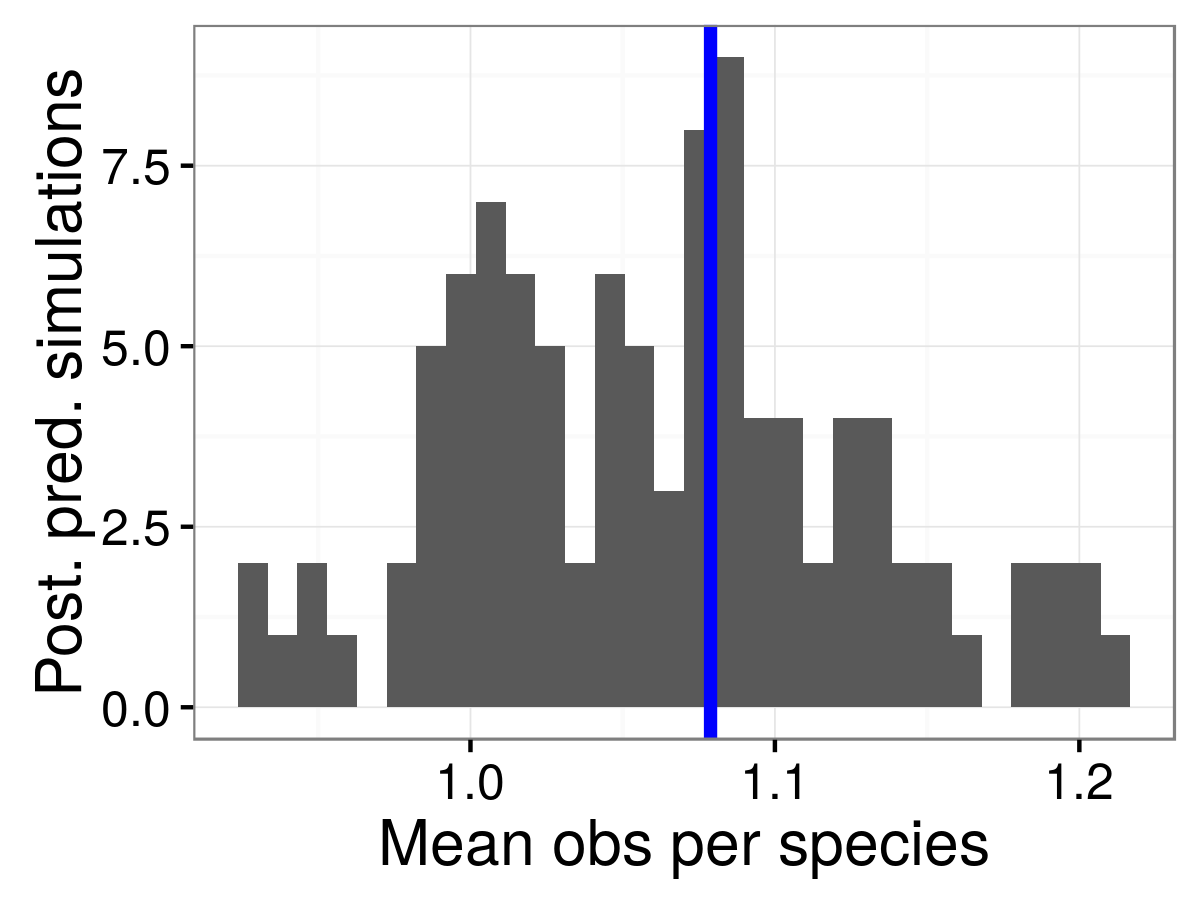
\includegraphics[width=\textwidth,height=0.3\textheight,keepaspectratio=true]{figure/pred_occ_bd}
  \caption[Posterior predictive check of average occurrence]{Comparison of the average observed number of occurrences per species (blue line) to the average number of occurrences from 100 posterior predictive datasets using the posterior estimates from the model used in this study. Adequate fit is indicated by the observed value of the test statistic being in the middle of the distribution of those calculated from the simulations.}
  \label{fig:ppc}
\end{figure}


% observation process
%   time
Log-odds of observing a species given that it is present varies greatly with time (Fig. \ref{fig:time_observe}) with lowest log-odds of observation being during the Gerigian and Harrisonian land-mammal ages. It is important to note, however, that all land-mammal ages with log-odds of observation greater than 2 have very high probabilities of observation, which means that while there may be large differences in log-odds of observation between land-mammal ages this may not translate to substantial difference in the probability of observation.
\begin{figure}[ht]
  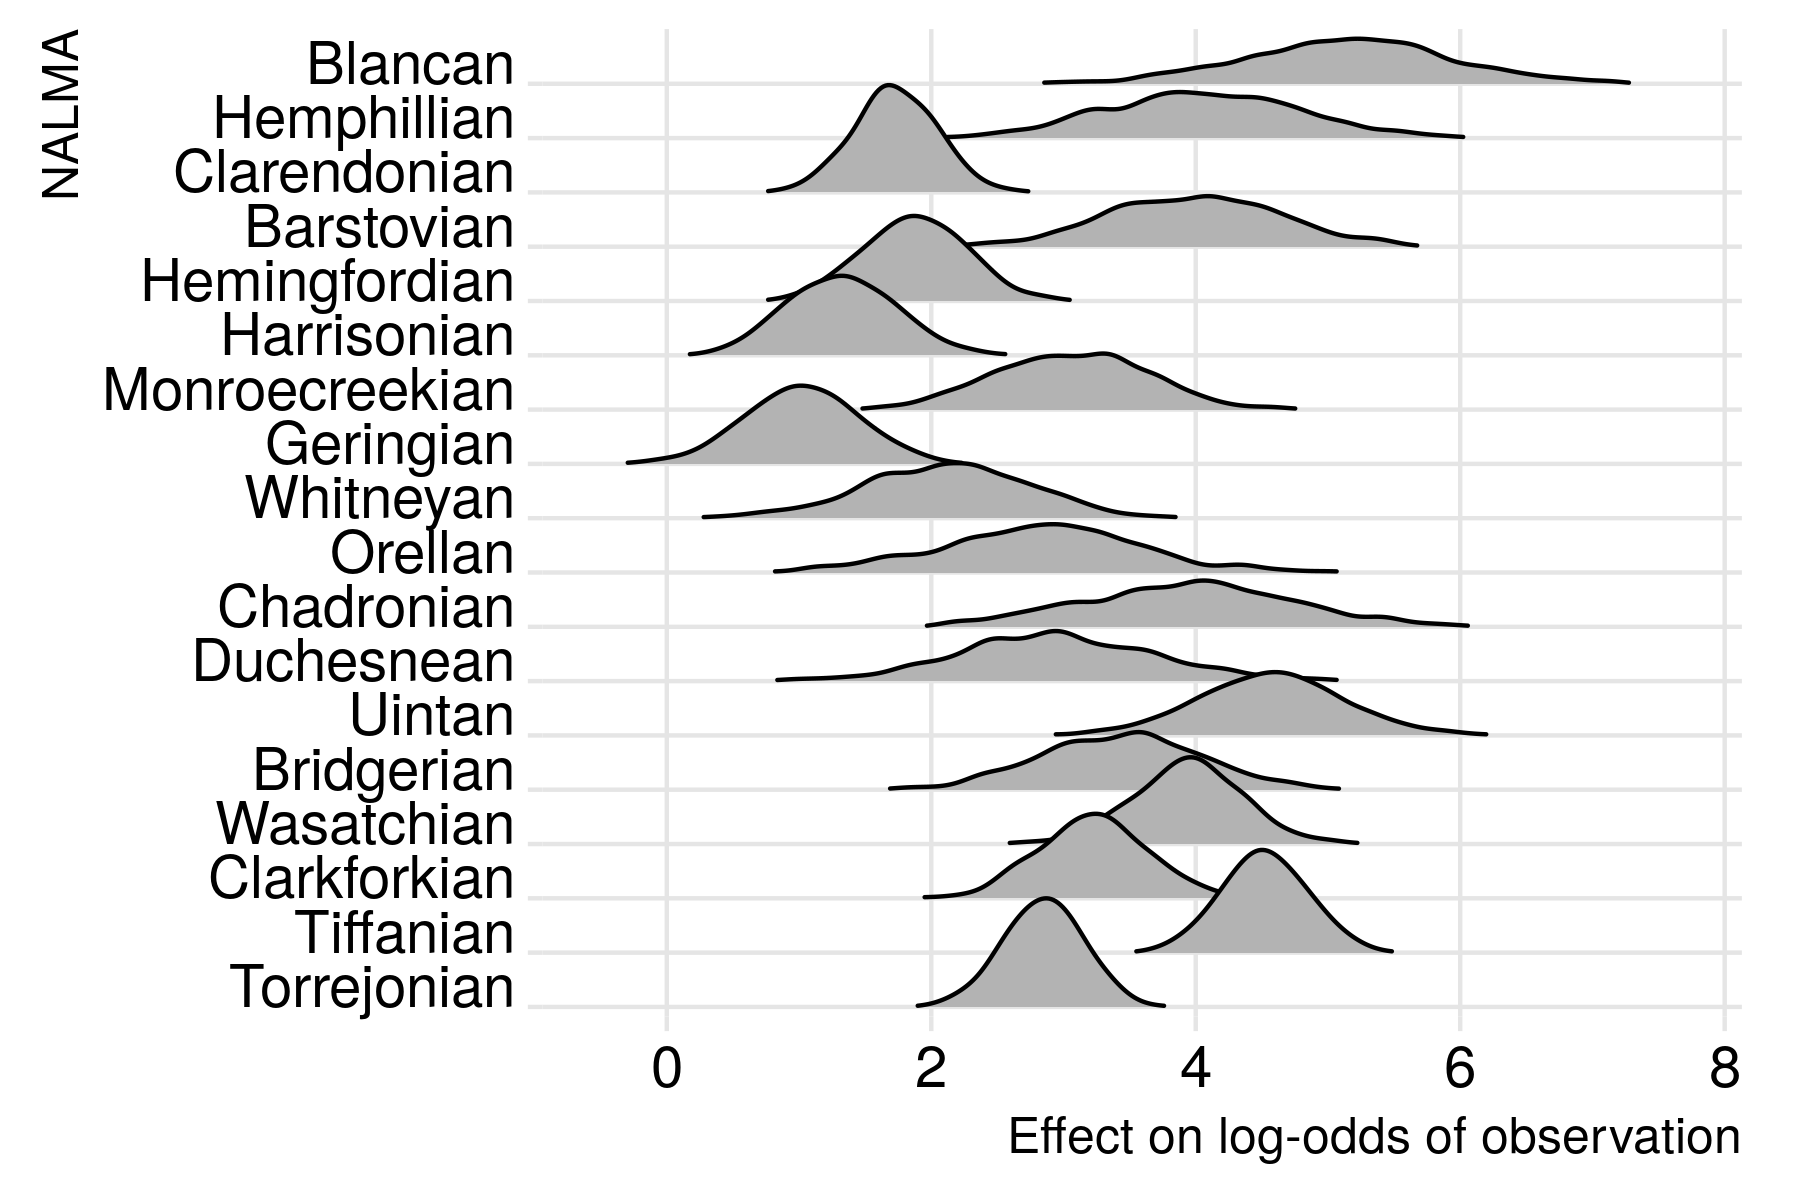
\includegraphics[width=\textwidth,height=0.4\textheight,keepaspectratio=true]{figure/time_observation}
  \caption{Ridgeline density plots of the estimates for the log-odds of observation from the time-varying intercept term. Each of the named time units are North American land-mammal ages. The oldest land-mammal age is at the bottom of the stack and the youngest is at the top.}
  \label{fig:time_observe}
\end{figure}

%   functional group
There is little variance in the effect of functional group on the log-odds of observing a species that is present (Fig. \ref{fig:fg_observe}). The only functional group with substantially less than expected log-odds of observation is scansorial insectivores, indicating that the fossil record of this group is the least complete of all the functional groups studied. Few functional groups have marginally better than expected log-odds of observation, the other insectivorous functional groups have marginally greater than average log-odds of observation; this is also the case for plantigrade omnivores. These results indicate that the observation histories of these functional groups are expected to be complete than most other functional groups. However, it is important to note that for many functional groups, their estimated log-odds of observation are poorly constrained with great uncertainty indicating little structure in how log-odds of observation varies between functional groups (Fig. \ref{fig:fg_observe}).
\begin{figure}[ht]
  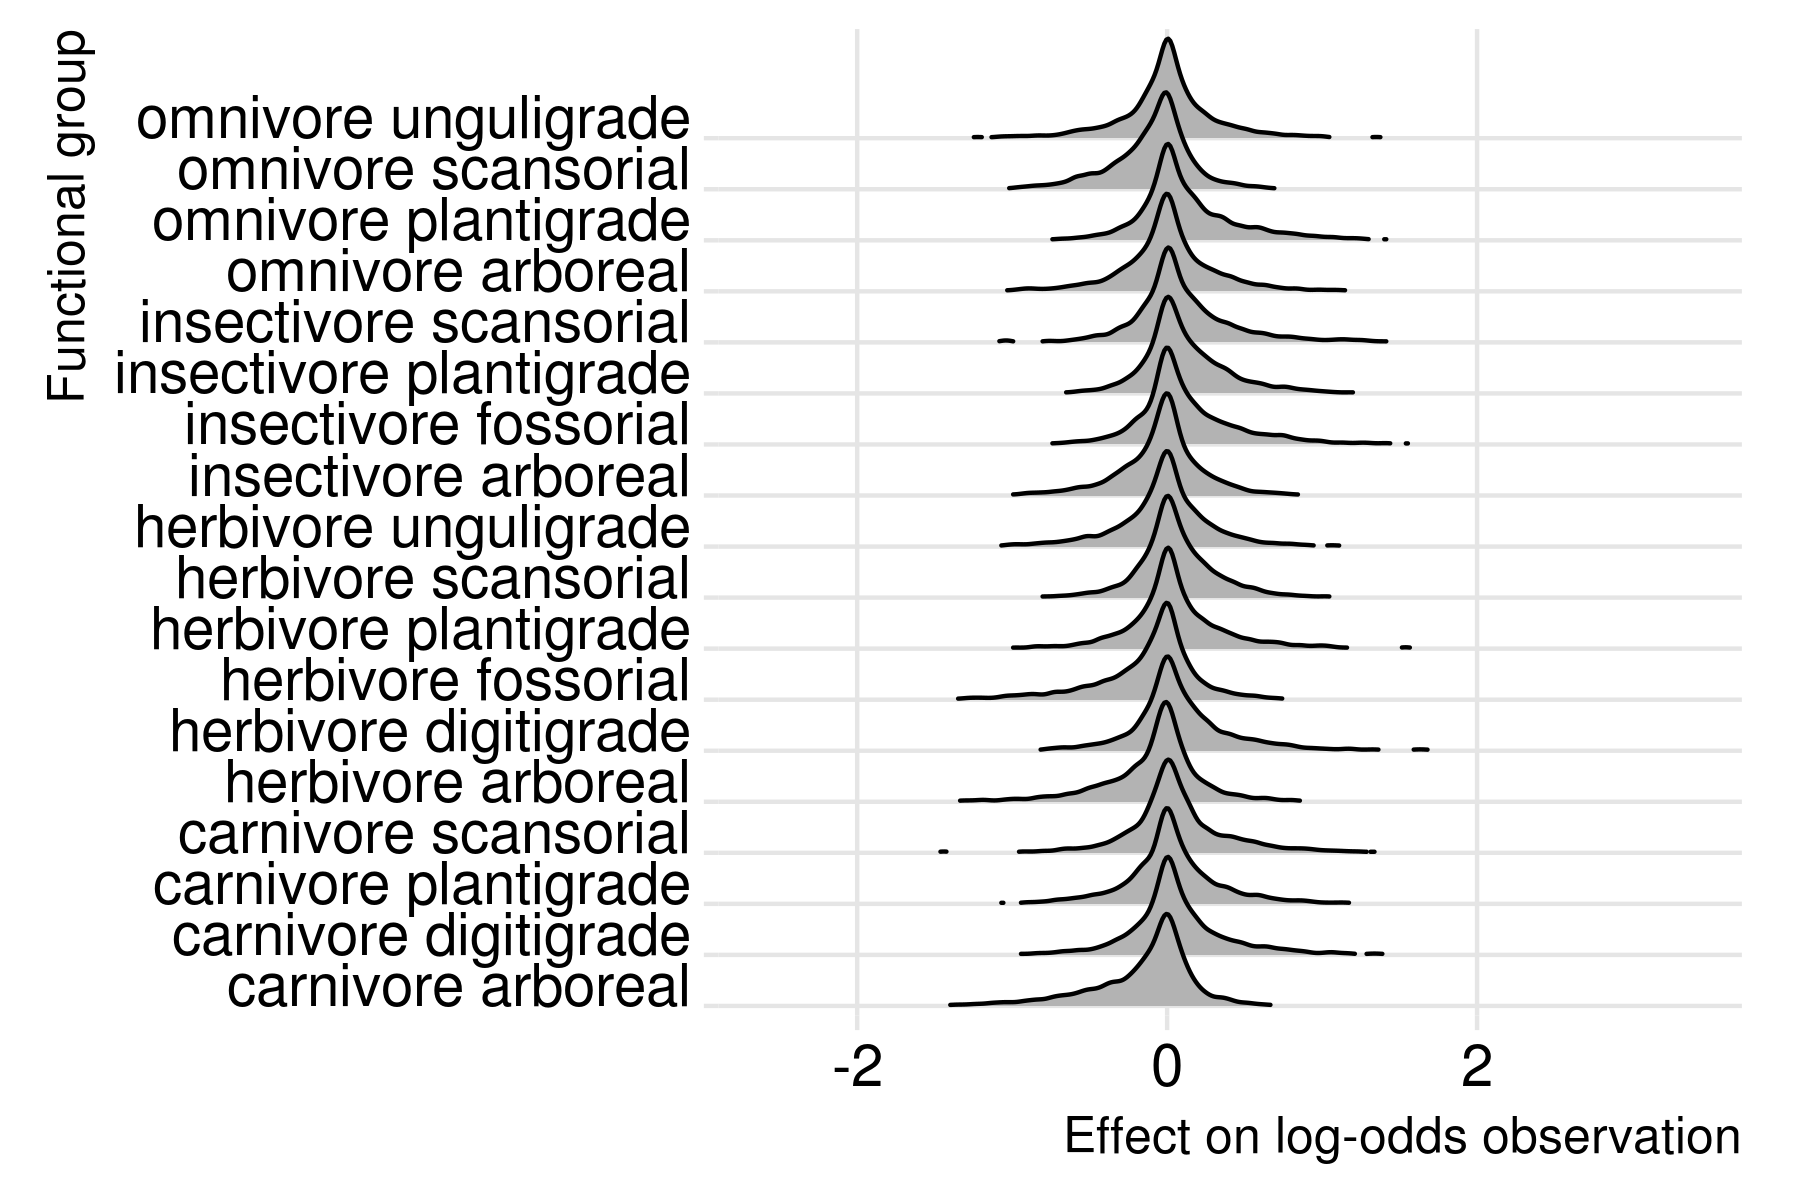
\includegraphics[width=\textwidth,height=0.4\textheight,keepaspectratio=true]{figure/ecotype_observation}
  \caption{Ridgeline density plots of the estimates of the effect of functional group on log-odds of observation. Each of the rows correspond to a different functional group as indicated by the dietary and locomotor category combination.}
  \label{fig:fg_observe}
\end{figure}

%   mass
Species mass is found to have a positive effect on probability of observing a species that is present (Fig. \ref{fig:mass_observe}). This result indicates that species with greater than average mass are expected to have more complete observation histories than species with less than average mass. However, this estimate does not translate to substantial differences in the estimated probability of observation because observation probability is so high for most of the Cenozoic (Fig. \ref{fig:time_observe}). In fact, it is only when land-mammal age observation probability is low that the effect of mass is observable. It is important to remember the effect of mass on observation was considered constant over time and that all differences observation probability between land-mammal ages is driven by variation over time. When log-odds of observation is high, differences due to covariate effects translate to very small differences in actual probability. % change this to just a single response curve? i like that i can visualize how little mass matters depending on overall prob of observation
\begin{figure}[ht]
  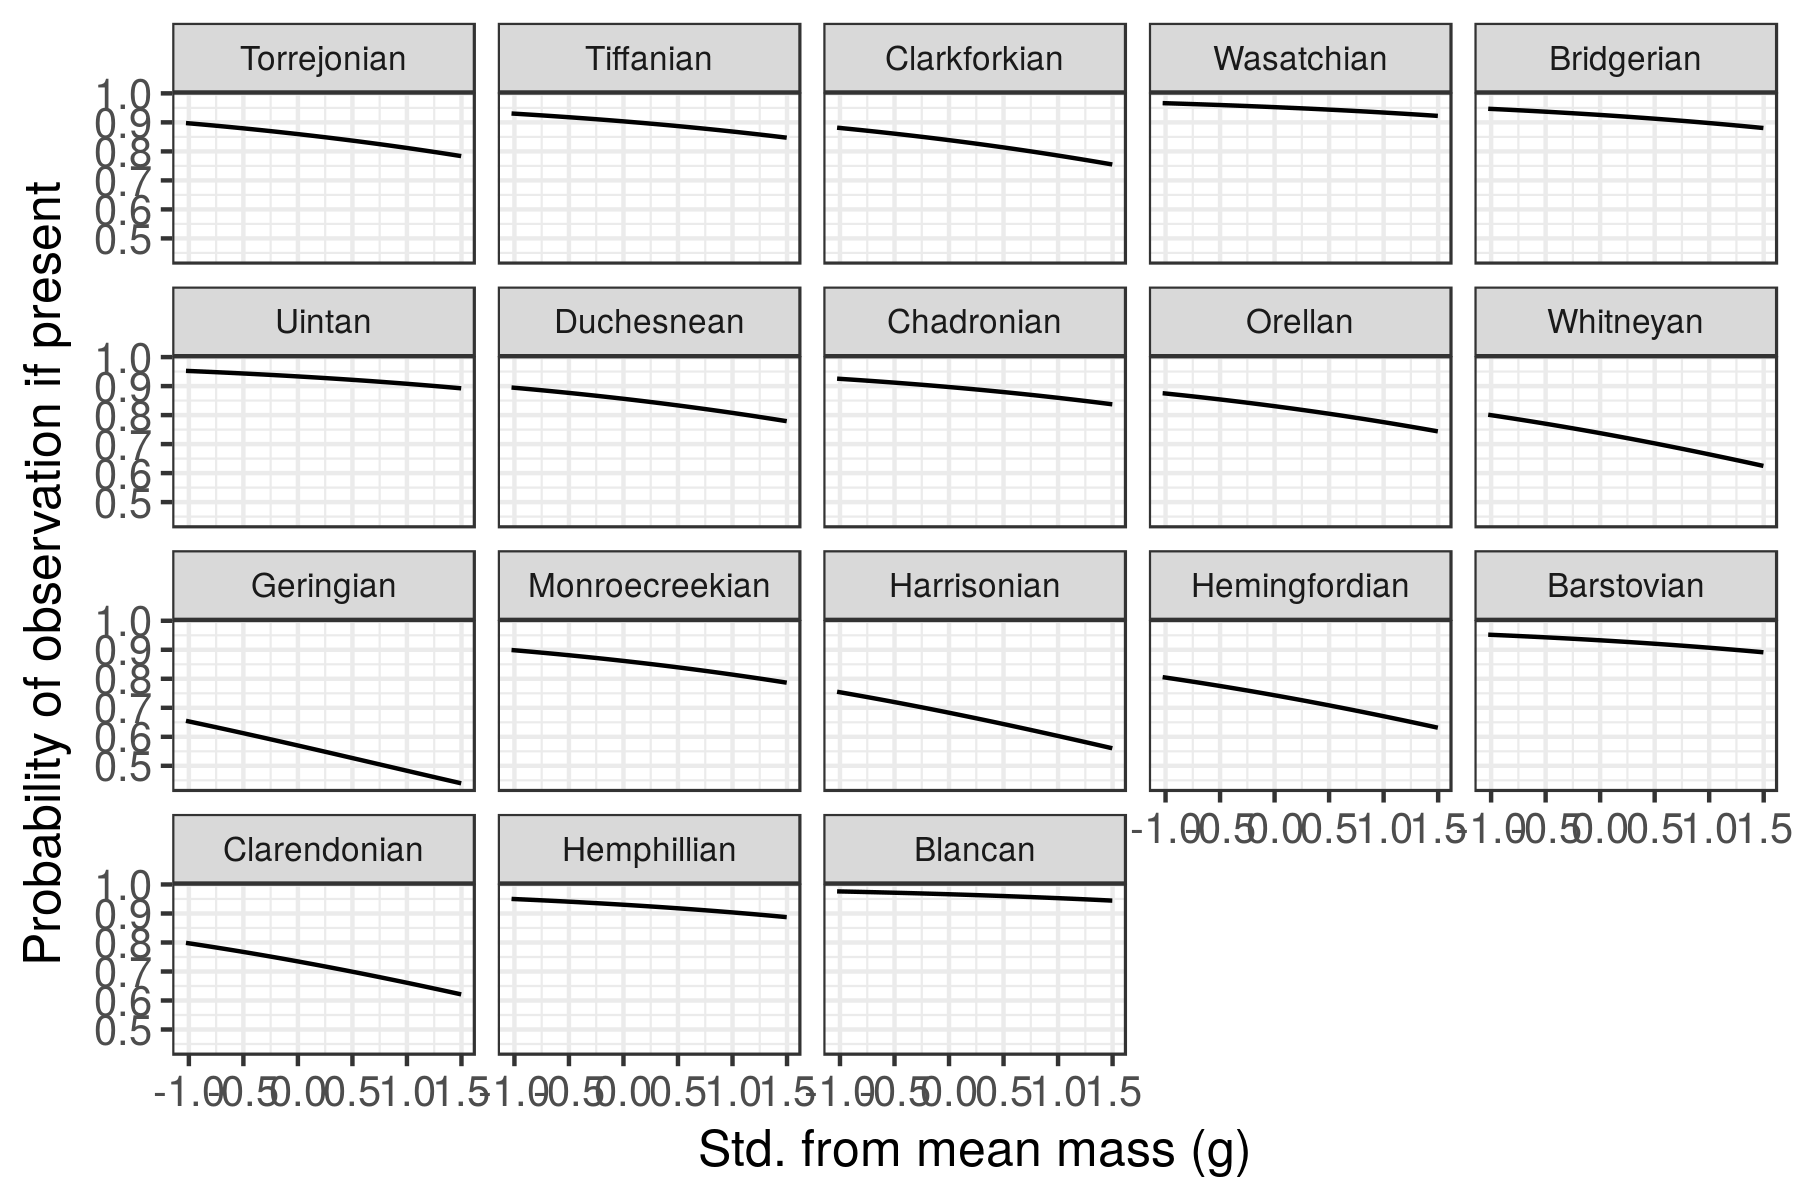
\includegraphics[width=\textwidth,height=0.4\textheight,keepaspectratio=true]{figure/mass_on_pres_bd}
  \caption[Estimates of the effect of mass on observation probability]{Estimates of the effect of species mass on probability of sampling a present species (\(p\)). Mass has been log-transformed, centered, and rescaled; this means that a mass of 0 corresponds to the mean of log-mass of all observed species and that mass is in standard deviation units. Probability of observation is presented for each of the NALMAs where the differences in mean probability of observation are due to variation between the time units (Fig. \ref{fig:time_observe}).}
  \label{fig:mass_observe}
\end{figure}


% origination
%   individual-level
%     FG time series
Origination probability varies greatly among functional groups with each functional group exhibiting a unique time series with a few shared features (Fig. \ref{fig:eco_origin}). When origination probability is below 0.50 this means that few if any new species of that functional group are entering the species pool, and when origination probability is greater than 0.50 new species of that functional group are probably entering the species pool. Finally, if origination probability is approximately 0.50, this indicates that it is equally likely that a new species is entering the species pool as that it is not. The slope of origination probability time-series is also very revealing; when the slope of the time series is positive then new species are being continually being added to the species pool, and when the slope is negative then the number of new species entering the pool is decreasing with time.

Most of the functional groups have peak origination probability at the present (Fig. \ref{fig:eco_origin}); new species in these functional groups are continually being added to the species pool. In the case of some functional groups,  such as digitigrade carnivores and fossorial herbivores, this is the culmination of those groups continued growth in the species pool. For other functional groups, such as arboreal herbivores, this peak is a reversal from previously relatively low origination probability; this indicates an expansion of these functional groups following a retraction.

Five of the functional groups have peak origination probabilities not at the present: arboreal carnivores, arboreal insectivores, plantigrade insectivores, scansorial insectivores, and unguligrade omnivores. The arboreal functional groups reach peak origination probability in the Paleogene, after which their origination probabilities approach and remain at 0.50, reflecting the loss of these functional groups from the species pool as origination probability never again increases. Additionally, the uncertainty surrounding in the estimates of origination probability is very large, especially in the Neogene. Large uncertainty in probabilities can reflect complete separation which results from that functional group leaving the species pool and it's (lack of) occurrence is without ambiguity CITATION. The patterns evinced by the other functional groups have similar properties but reach peak origination probability early in the Neogene. Interestingly, origination probability of scansorial insectivores has effectively two peaks, once in the late Paleogene and again in the early Neogene. Additionally, as will be discussed later in the context of standing diversity, all five of these functional groups decrease in diversity through the Cenozoic. 
\begin{figure}[ht]
  \centering
  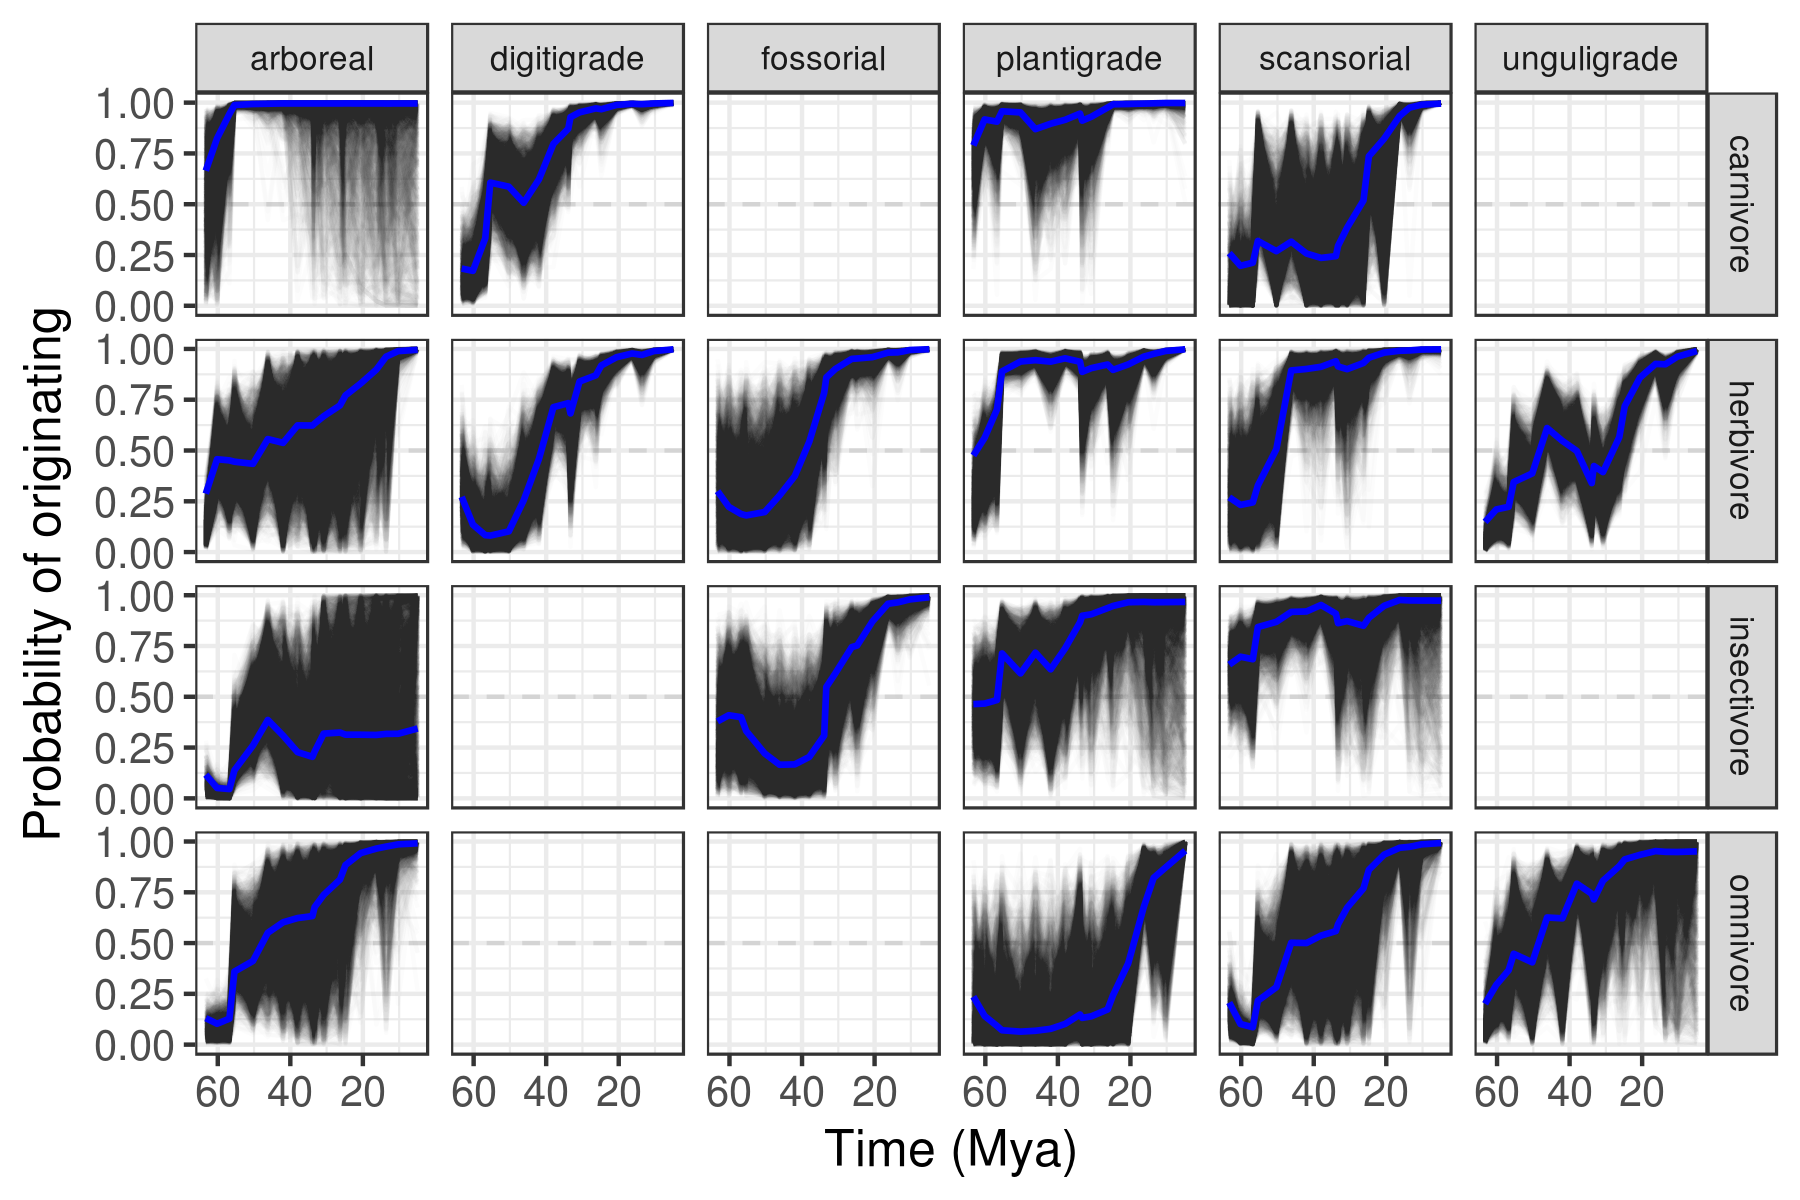
\includegraphics[width=\textwidth,height=0.4\textheight,keepaspectratio=true]{figure/ecotype_origin_bd}
  \caption[Estimates of functional group origination probability]{Probability of a mammal functional origination at each time point. Each panel depicts 100 time-series sampled from the model's posterior. The blue line is the mean origination probability as predicted by the group-level predictors. The columns are by locomotor category and rows by dietary category; their intersections are the observed and analyzed ecotypes. }
  \label{fig:eco_origin}
\end{figure}

%     order effect
Origination probability varies greatly amongst mammal orders (Fig. \ref{fig:order_origin}). These estimates reflect differences origination probability as well as the relative rarity of that order in the fossil record; if members of that order appear infrequently, they must have lower probability of origination. Orders with greater than average log-odds of origination include Multituberculata, Dinocerata, Didelphimorphia, Creodonta, Condylarthra, Cimolesta, and Acreodi. These orders are major components of the Paleogene fossil record. Orders with lower than average log-odds of origination include Rodentia, Pilosa, Lagomorpha, Eulipotyphyla, Cingulata, Carnivora, and Artiodactyla. These orders are characterized by small body size or primarily Neogene records. Additionally, the variance between orders is vary large ranging from -3 to 3 log-odds of origination; this large of variance reflects how species within these orders have very different patterns of origination independent from their origination based on functional ecology (Fig. \ref{fig:eco_origin}).
\begin{figure}[ht]
  \centering
  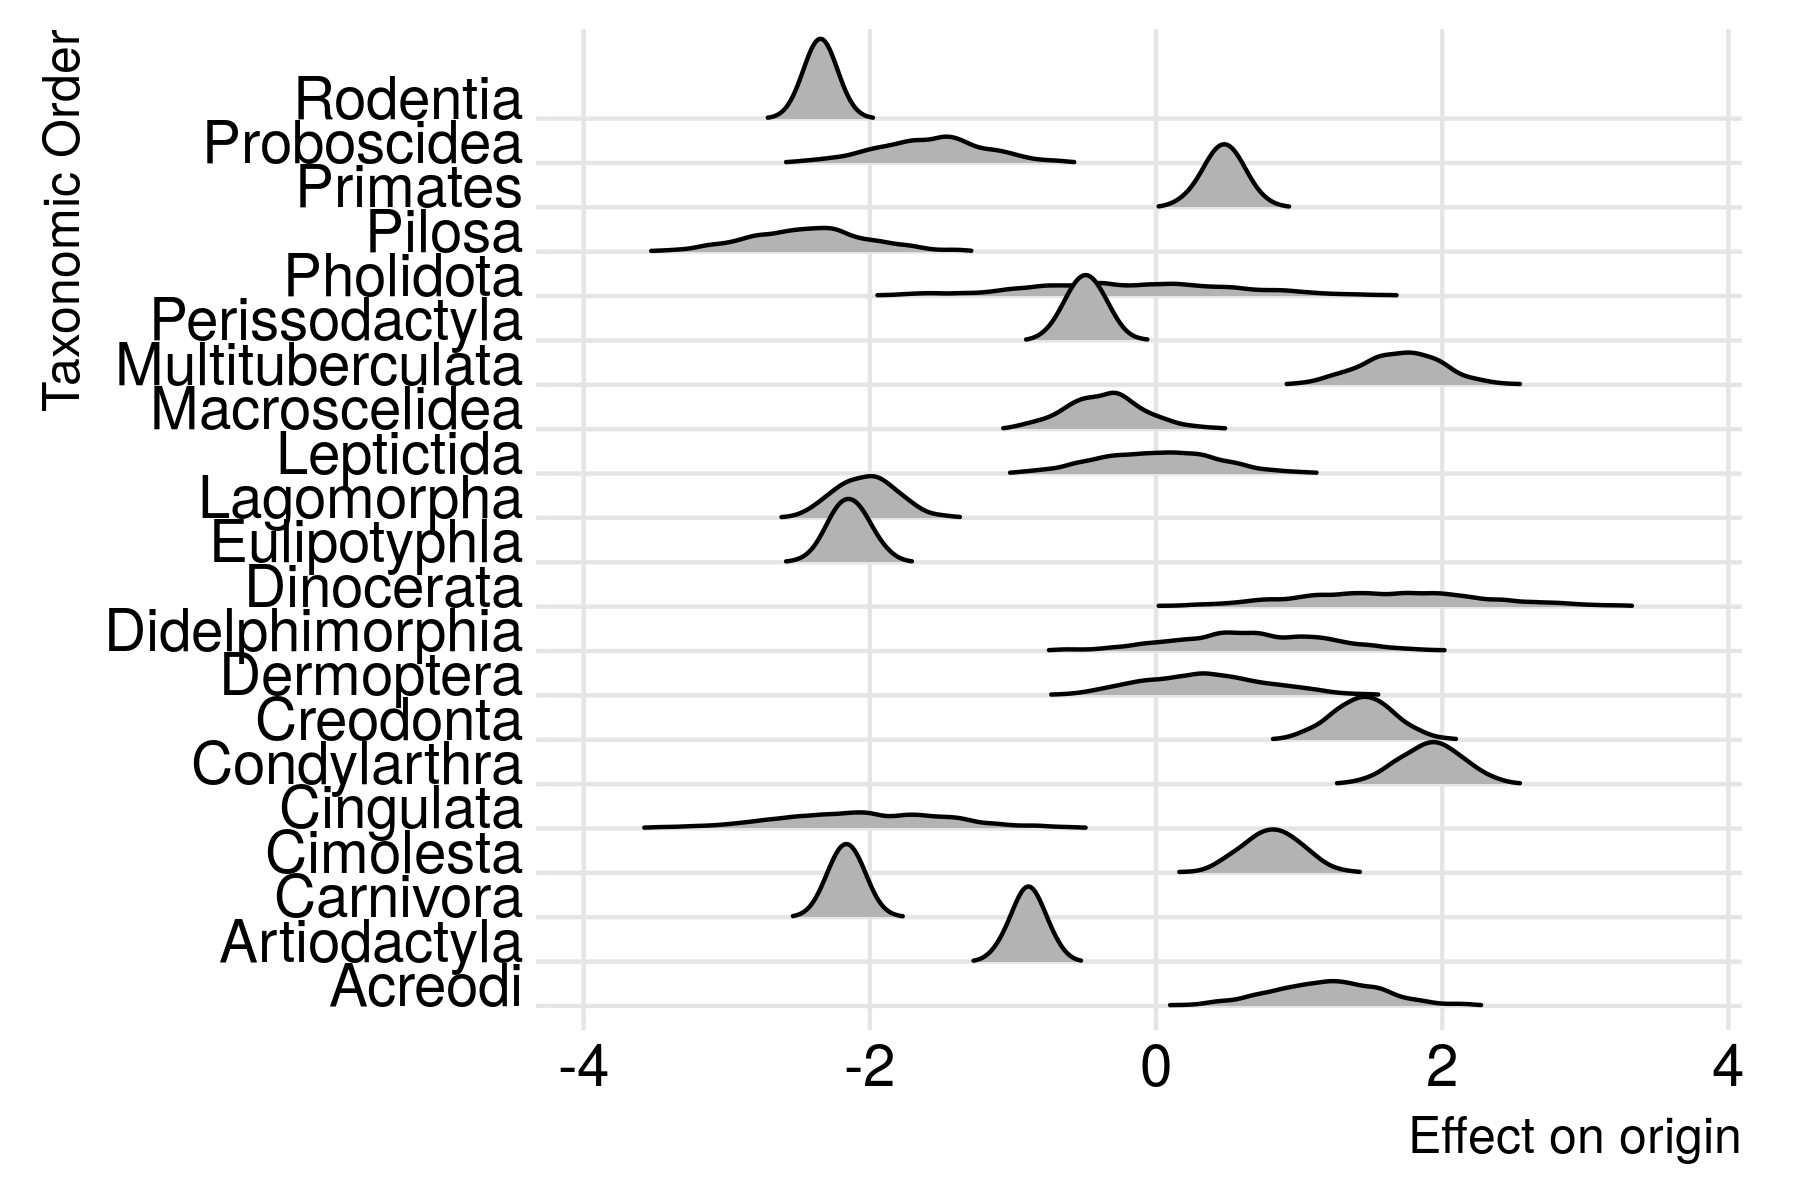
\includegraphics[width=\textwidth,height=0.4\textheight,keepaspectratio=true]{figure/order_origin_bd}
  \caption{Differences in log-odds of origination based on mammal orders. Positive values correspond to greater log-odds origination than average, while negative values correspond to lower log-odds of origination than average. These estimates reflect the rarity of that order in the fossil record as well as differences in origination.}
  \label{fig:order_origin}
\end{figure}

%     mass effect
Species mass is estimated to have a negative relationship with origination probability (Fig. \ref{fig:mass_origin}). This result means that species with greater than average mass have a lower probability of originating than species with a below average mass. This result is sensible given the left-skewed distribution of mammal species body sizes where large body sizes form the right-hand tail. There are fewer large body-sized mammals which have originated than small body sized mammals. Interestingly, many of the orders with small body sizes (e.g. Rodentia, Lagomorpha) have below average probabilities of originating (Fig. \ref{fig:order_origin}); while not completely kosher, when this result is considered together with the effect of mass on origination these effects could be counteracting each other. These results continue to add to the understanding of the heterogeneity and nuance associated with species origination dynamics.
\begin{figure}[ht]
  \centering
  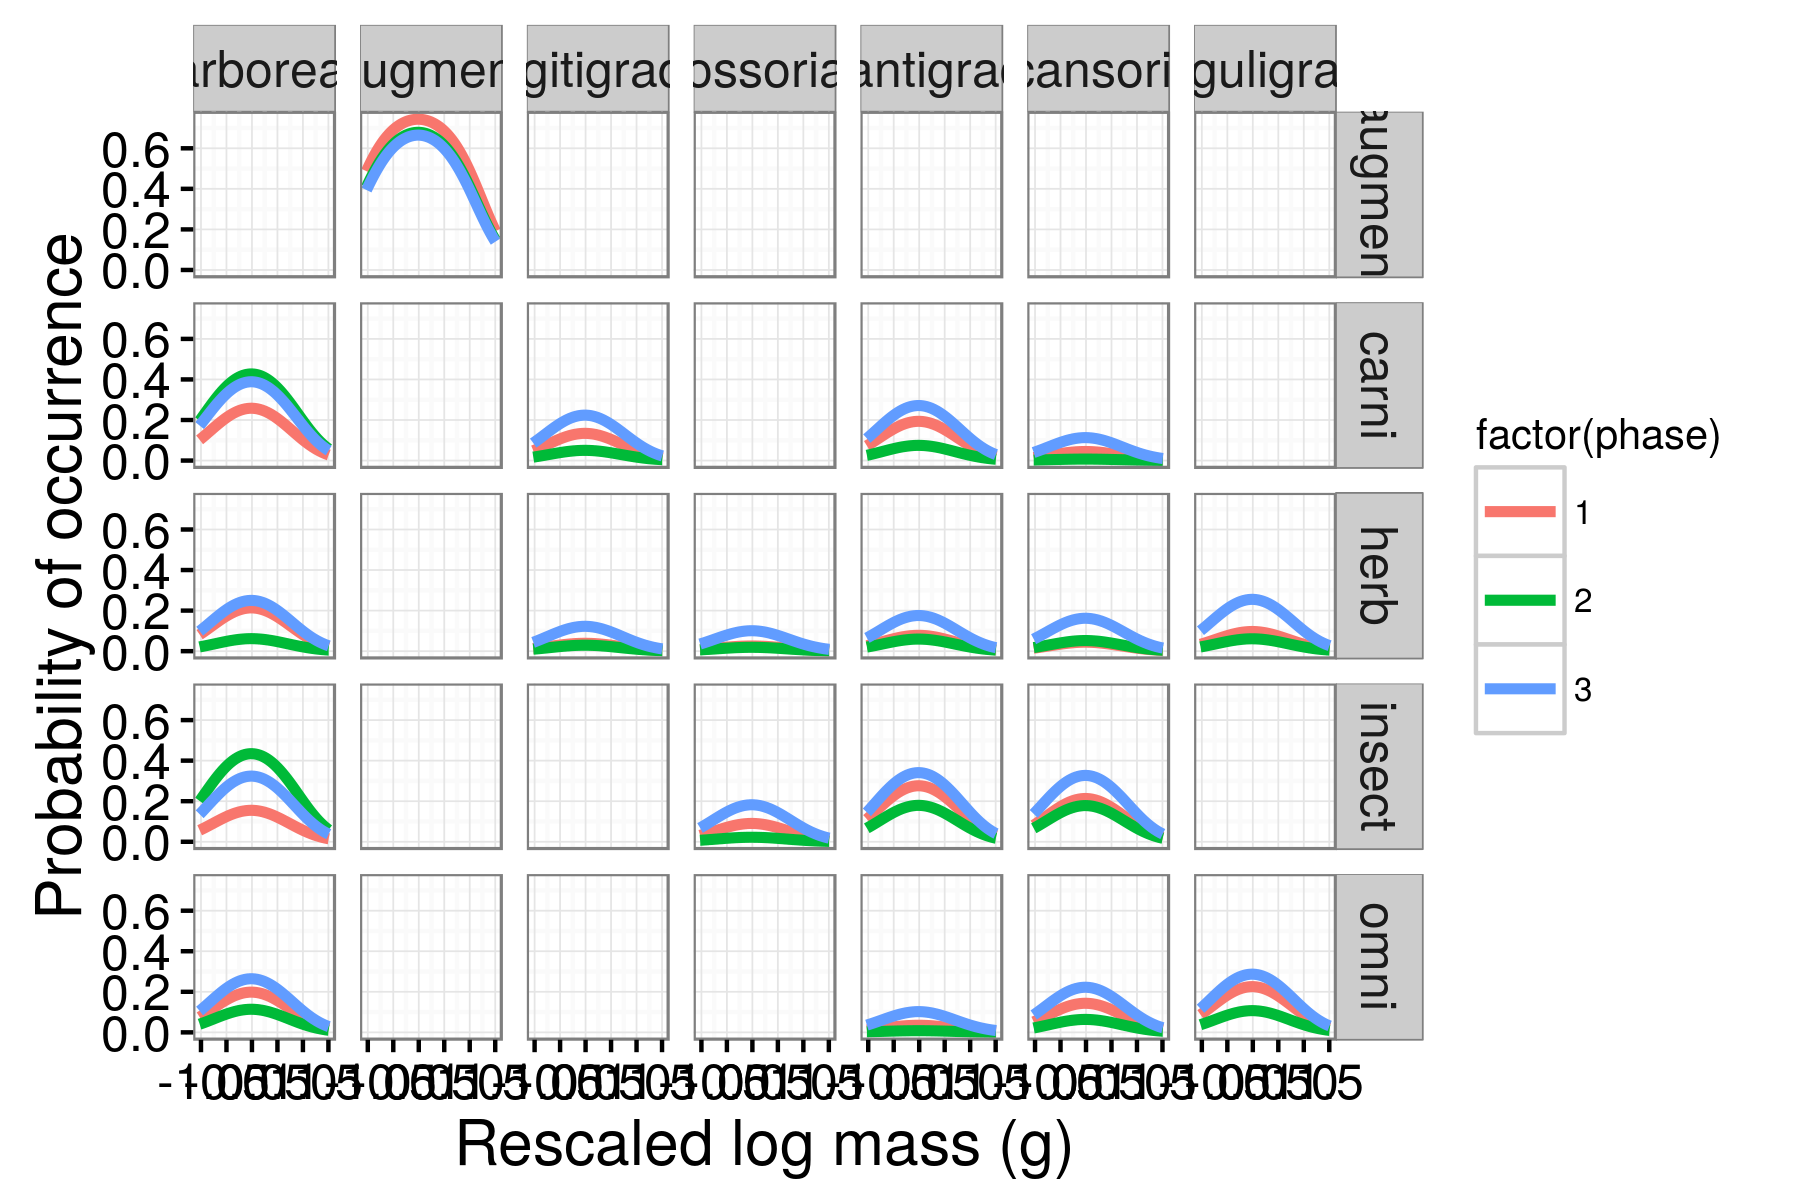
\includegraphics[width=\textwidth,height=0.4\textheight,keepaspectratio=true]{figure/mass_on_origin_bd}
  \caption[Effect of mass on probability of species origination as estimated from the birth-death model]{Mean estimate of the effect of species mass on the probability of a species originating for each of the three plant phases. The effect of mass is considered constant over time and that the only aspect of the model that changes with plant phase is the intercept of the relationship between mass and origination. The three plant phases are indicated by the color of the line. Mass has been log-transformed, centered, and rescaled; this means that a mass of 0 corresponds to the mean of log-mass of all observed species and that mass is in standard deviation units. For clarity, only the mean estimates of the effects of mass and plant phase are plotted.}
  \label{fig:mass_origin}
\end{figure}

%   group-level
%     temperature and plant phase
\begin{figure}[ht]
  \centering
  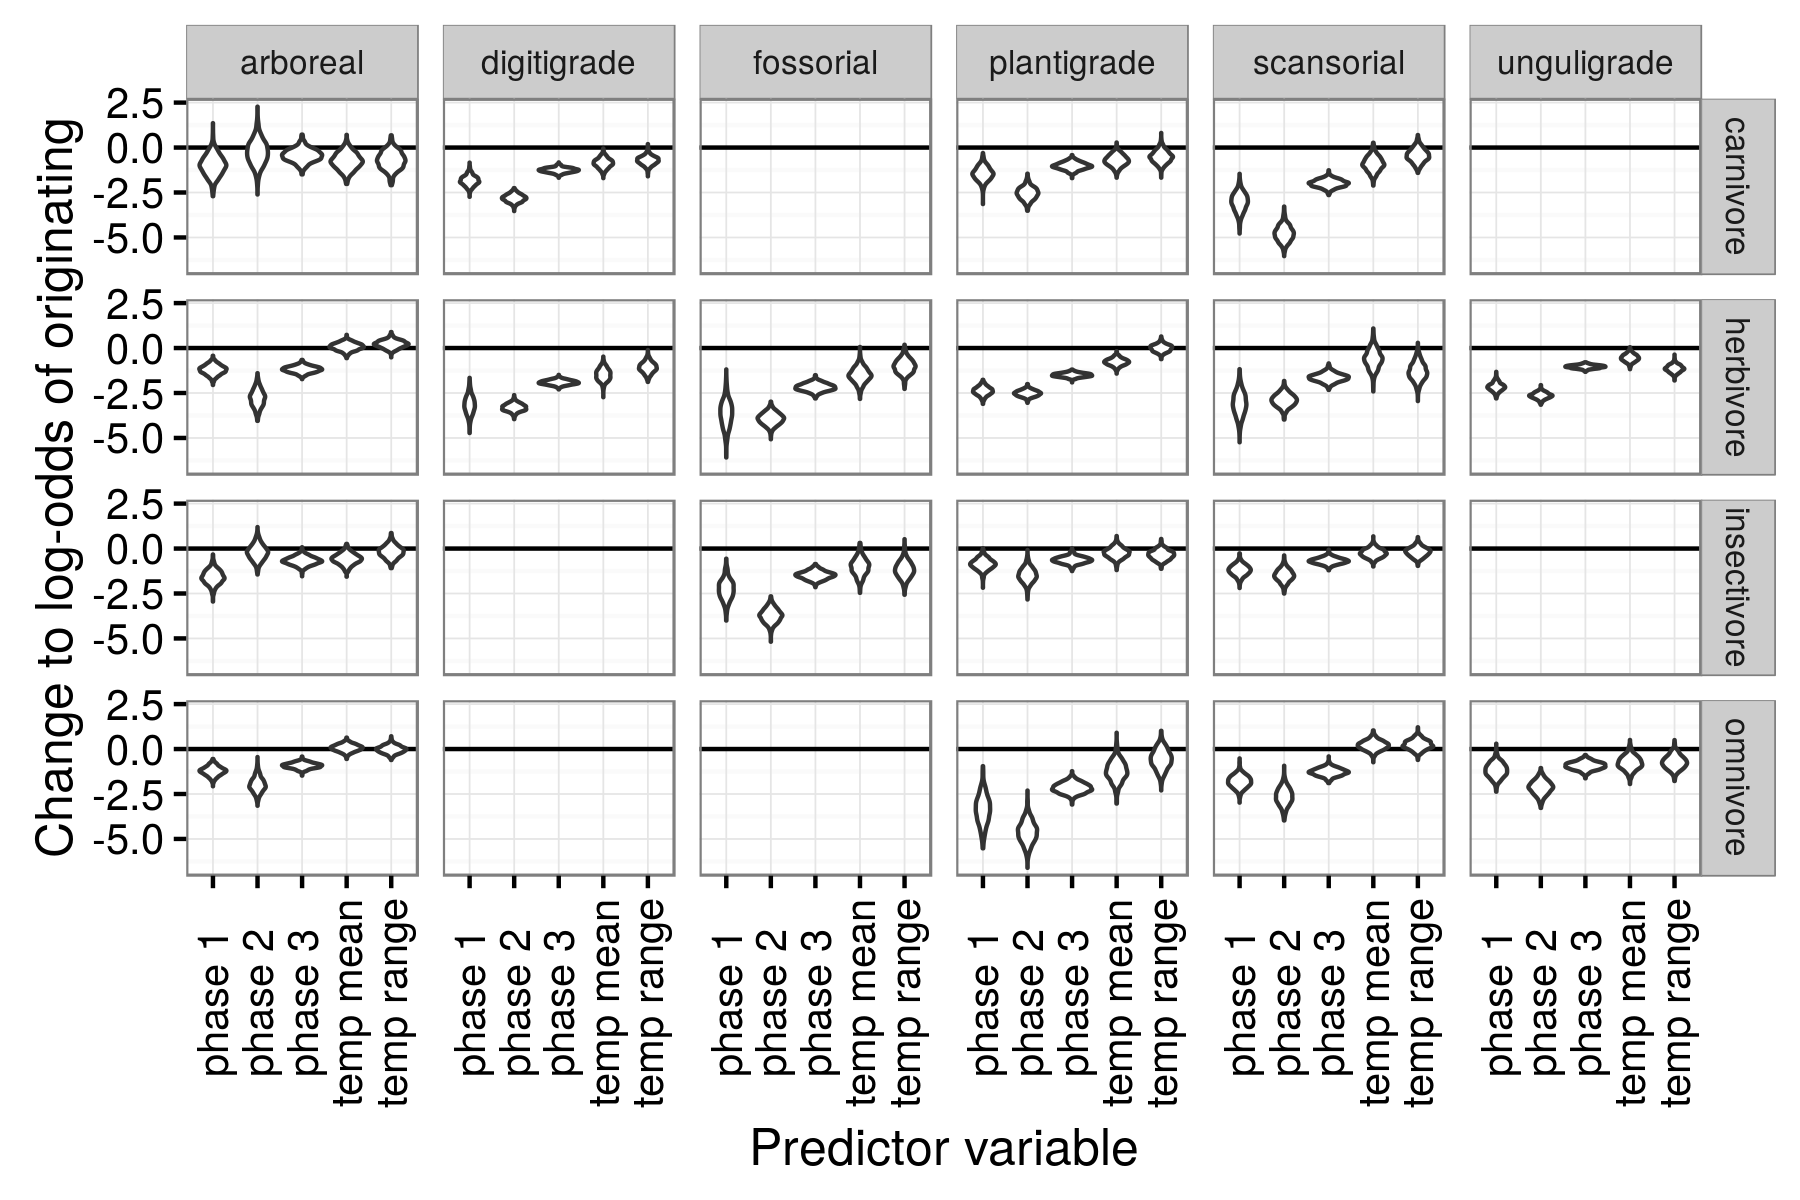
\includegraphics[width=\textwidth,height=0.4\textheight,keepaspectratio=true]{figure/group_on_origin_bd}
  \caption[Effects of group-level covariates on log-odds of ecotype origination as estimated from the birth-death model]{Estimated effects of the group-level covariates describing environmental context on log-odds of species origination. These estimates are from the birth-death model. What is plotted is a violin of the distribution of 1000 samples from the approximate posterior. The effect of plant phase graphed here is calculated as Phase 1\( = \gamma_{phase\ 1}\), Phase 2\( = \gamma_{phase\ 1} + \gamma_{phase\ 2}\), and so on.} 
  \label{fig:group_origin_bd}
\end{figure}

\begin{table}[ht]
  \centering
  \caption[Posterior probablity estimates of differences in origination by plant phase]{Posterior probability of the differences in the log-odds of an ecotype originating based on plant phase.} 
  \label{tab:origin_plant}
  \begin{tabular}{ l r r r }
    \hline
    & P(Eo.Mi $>$ 0) & P(Pa.Eo $>$ 0) & P(Eo.Mi $>$ Pa.Eo) \\ 
    \hline
    arboreal carnivore & 0.575 & 0.447 & 0.598 \\ 
    digitigrade carnivore & 0.976 & 0.017 & 0.998 \\ 
    plantigrade carnivore & 0.857 & 0.780 & 0.578 \\ 
    scansorial carnivore & 0.768 & 0.154 & 0.889 \\ 
    arboreal herbivore & 0.318 & 0.357 & 0.428 \\ 
    digitigrade herbivore & 1.000 & 0.161 & 0.995 \\ 
    fossorial herbivore & 0.999 & 0.353 & 0.926 \\ 
    plantigrade herbivore & 1.000 & 0.304 & 0.998 \\ 
    scansorial herbivore & 0.999 & 0.108 & 0.998 \\ 
    unguligrade herbivore & 0.000 & 0.000 & 0.100 \\ 
    arboreal insectivore & 0.364 & 0.003 & 0.857 \\ 
    fossorial insectivore & 0.645 & 0.341 & 0.708 \\ 
    plantigrade insectivore & 0.794 & 0.148 & 0.881 \\ 
    scansorial insectivore & 0.916 & 0.235 & 0.940 \\ 
    arboreal omnivore & 0.590 & 0.006 & 0.882 \\ 
    plantigrade omnivore & 0.524 & 0.209 & 0.762 \\ 
    scansorial omnivore & 0.713 & 0.027 & 0.938 \\ 
    unguligrade omnivore & 0.888 & 0.127 & 0.960 \\ 
    \hline
  \end{tabular}
\end{table}

\begin{table}[ht]
  \centering
  \caption[Posterior probablity of effects of temperature on origination]{Posterior probability that the effects of the two temperature covariates on the log-odds of an ecotype origination are greater than 0. What is estimated is the probability that these estimates are greater than 0; high or low probabilities indicate the ``strength'' of the covariate in that direction (positive and negative, respectively). These estimates are from the birth-death model.}
  \label{tab:origin_temp}
  \begin{tabular}{ l r }
    \hline
    & \(P(\gamma_{temp\ mean} > 0)\) \\
    \hline
    arboreal carnivore & 0.355 \\ 
    digitigrade carnivore & 0.001 \\ 
    plantigrade carnivore & 0.358 \\ 
    scansorial carnivore & 0.121 \\ 
    arboreal herbivore & 0.219 \\ 
    digitigrade herbivore & 0.045 \\ 
    fossorial herbivore & 0.067 \\ 
    plantigrade herbivore & 0.000 \\ 
    scansorial herbivore & 0.221 \\ 
    unguligrade herbivore & 0.339 \\ 
    arboreal insectivore & 0.027 \\ 
    fossorial insectivore & 0.219 \\ 
    plantigrade insectivore & 0.224 \\ 
    scansorial insectivore & 0.192 \\ 
    arboreal omnivore & 0.009 \\ 
    plantigrade omnivore & 0.087 \\ 
    scansorial omnivore & 0.035 \\ 
    unguligrade omnivore & 0.129 \\ 
    \hline
  \end{tabular}
\end{table}

%     correlation
\begin{figure}[ht]
  \centering
  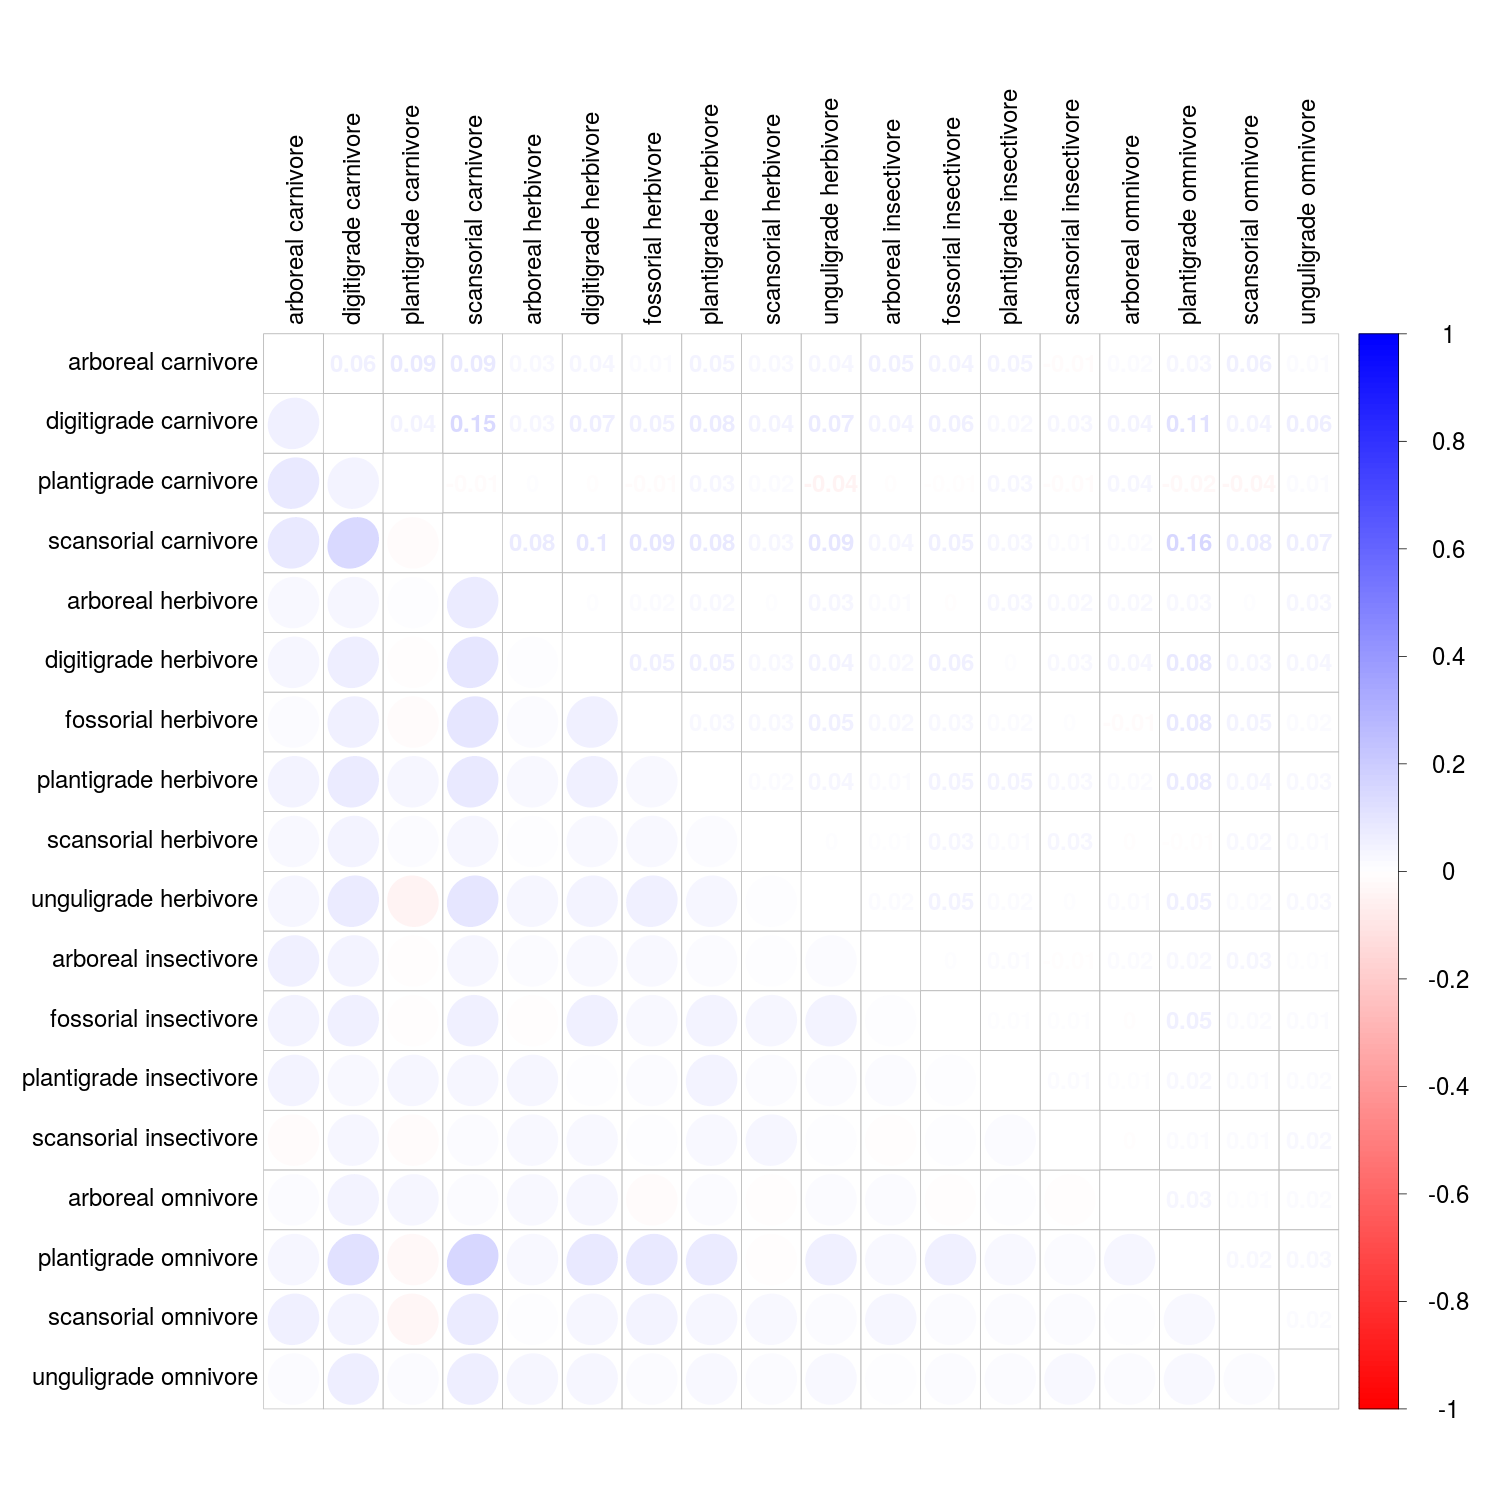
\includegraphics[width=\textwidth,height=\textheight,keepaspectratio=true]{figure/origination_correlation}
  \caption[Estimated correlations in origination probability between ecotypes]{Posterior mean estimates of the correlations in origination probability between the mammal ecotypes. The lower triangle of the matrix is populated with ellipses corresponding to the level of correlation between the two ecotypes, while the upper triangle of the matrix corresponds to the mean estimated correlation between ecotypes. Darker values correspond to a greater magnitude of correlation with blue values corresponding to a positive correlation and red values a negative correlation.}
  \label{fig:origin_corr}
\end{figure}





% survival
%   individual-level
%     FG time series
The survival probability time-series vary greatly between each of the functional groups with each exhibiting unique patterns (Fig. \ref{fig:eco_survival}). Interestingly, unlike origination probability (Fig. \ref{fig:eco_origin}), survival probability is frequently estimated estimated with considerable uncertainty. When survival probability is below 0.50 then a species that is present is unlikely to survive from one time unit to the next, while when survival probability is greater than 0.50 species can be expected to survive to the next time unit. Finally, when survival probability is approximately 0.50 then survival and extinction are equally likely. Overall, survival probability is rarely estimated to be greater than 0.50 with any certainty. This result is consistent with the average occurrence being \(<\)1.35 time unit per species which means that a plurality of species have only a single temporal occurrence (Fig. \ref{fig:ppc}).

The survival probability of many functional groups is frequently approximately 0.50, indicating extinction is frequently random with respect to functional group (Fig. \ref{fig:eco_survival}). For example, the survival probability scansorial canirvores is approximately 0.50 for the entire time series which indicates that there is no best or worst time for this functional groups survival. Similar patterns can be observed for mean survival probability of arboreal omnivores, fossorial insectivores, and plantigrade omnivores though all three of these groups have sudden drops in survival probability in approximately the last 10Mya.

Arboreal herbivores are the only functional group for which survival probability is approximately above 0.50 for the entire Cenozoic (Fig. \ref{fig:eco_survival}). This result indicates that when an arboreal herbivore species is present it is expected to survive from one time unit to the next. However, it is important to note that arboreal herbivores are estimated to have an origination probability below 0.50 for most of the Cenozoic. Together, these results mean that arboreal herbivore species are rare but are expected to survive from one time point to the next.

A common feature of multiple functional group's survival probability time-series is a peak in survival during the Neogene (Fig. \ref{fig:eco_survival}). In most cases, these peaks are estimated with little uncertainty which indicates how apparent this event is. Digitigrade carnivores, digitigrade herbivores, plantigrade herbivores, scansorial insectivores, unguligrade herbivores, and unguligrade omnivores all peak in survival probability at approximately 25Mya. This peak in survival means that species of these functional groups which are unlikely to go extinct at this point, potentially indicating favorable environmental conditions for these groups at the Paleogene-Neogene transition. Additionally, this peak does not coincide with the movement from one plant phase to another (Table \ref{tab:plant_def}). 
\begin{figure}[ht]
  \centering
  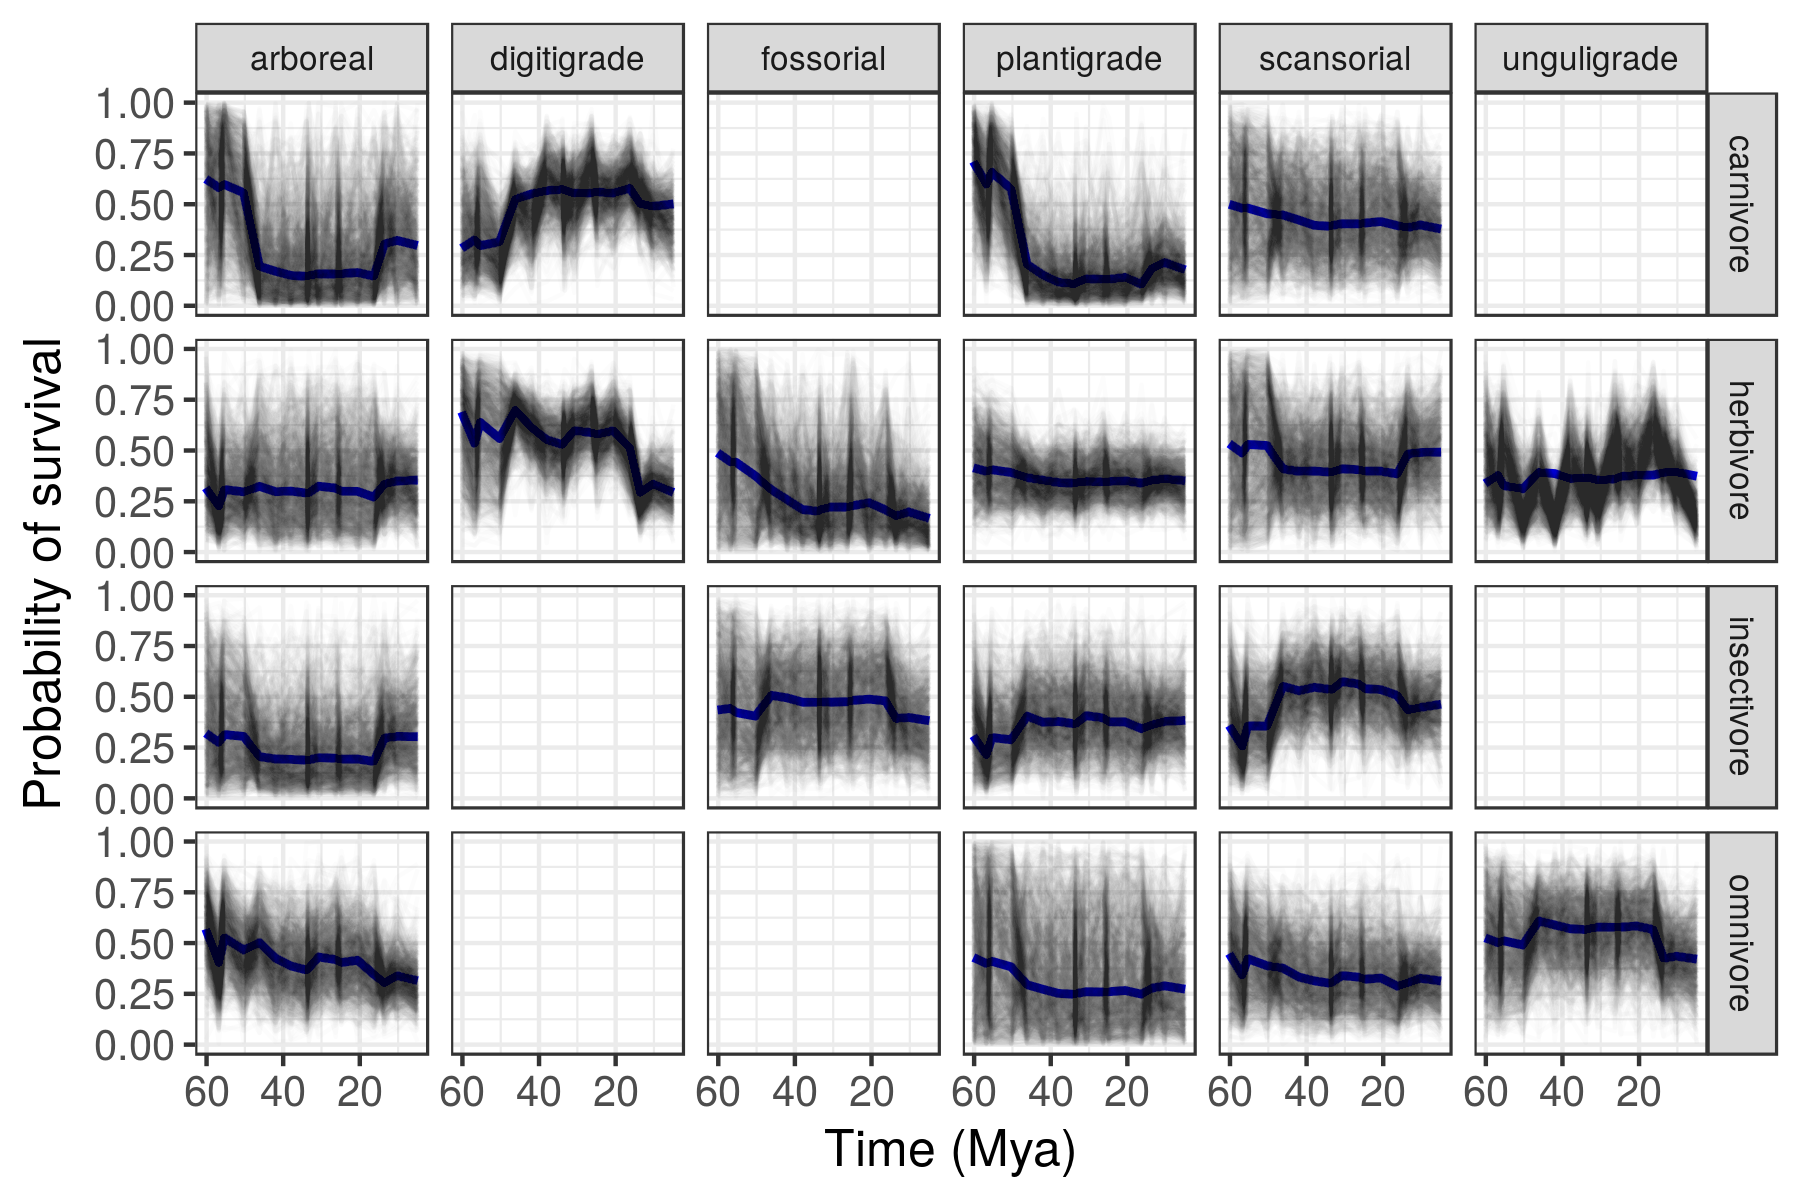
\includegraphics[width=\textwidth,height=0.4\textheight,keepaspectratio=true]{figure/ecotype_survival_bd}
  \caption[Ecotype survival probability estimated from the birth-death model]{Probability of a mammal ecotype survival probabilities at each time point as estimated from the birth-death model. Each panel depicts 100 random samples from the model's posterior. The columns are by locomotor category and rows by dietary category; their intersections are the observed and analyzed ecotypes. Panels with no lines are ecotypes not observed in the dataset.}
  \label{fig:eco_survival}
\end{figure}

%     order effect
The effect of order on survival probability has much lower variance (Fig. \ref{fig:order_surv}) than the effect of order on origination probability (Fig. \ref{fig:order_origin}. Primates, Multituberculata, Eulipotyphla, Dermoptera, Creodonta, Condylarthra, Carnivora, and Artiodactyla are estimated to have a lower than average survival probability which implies that species of these orders are expected to be present for a single time unit. Of these orders, Primates and Multituberculata are expected to have the lowest survival probability of all orders. The orders expected to have greater than average survival probability are Rodentia, Lagomorpha, and Didelphimorphia.
\begin{figure}[ht]
  \centering
  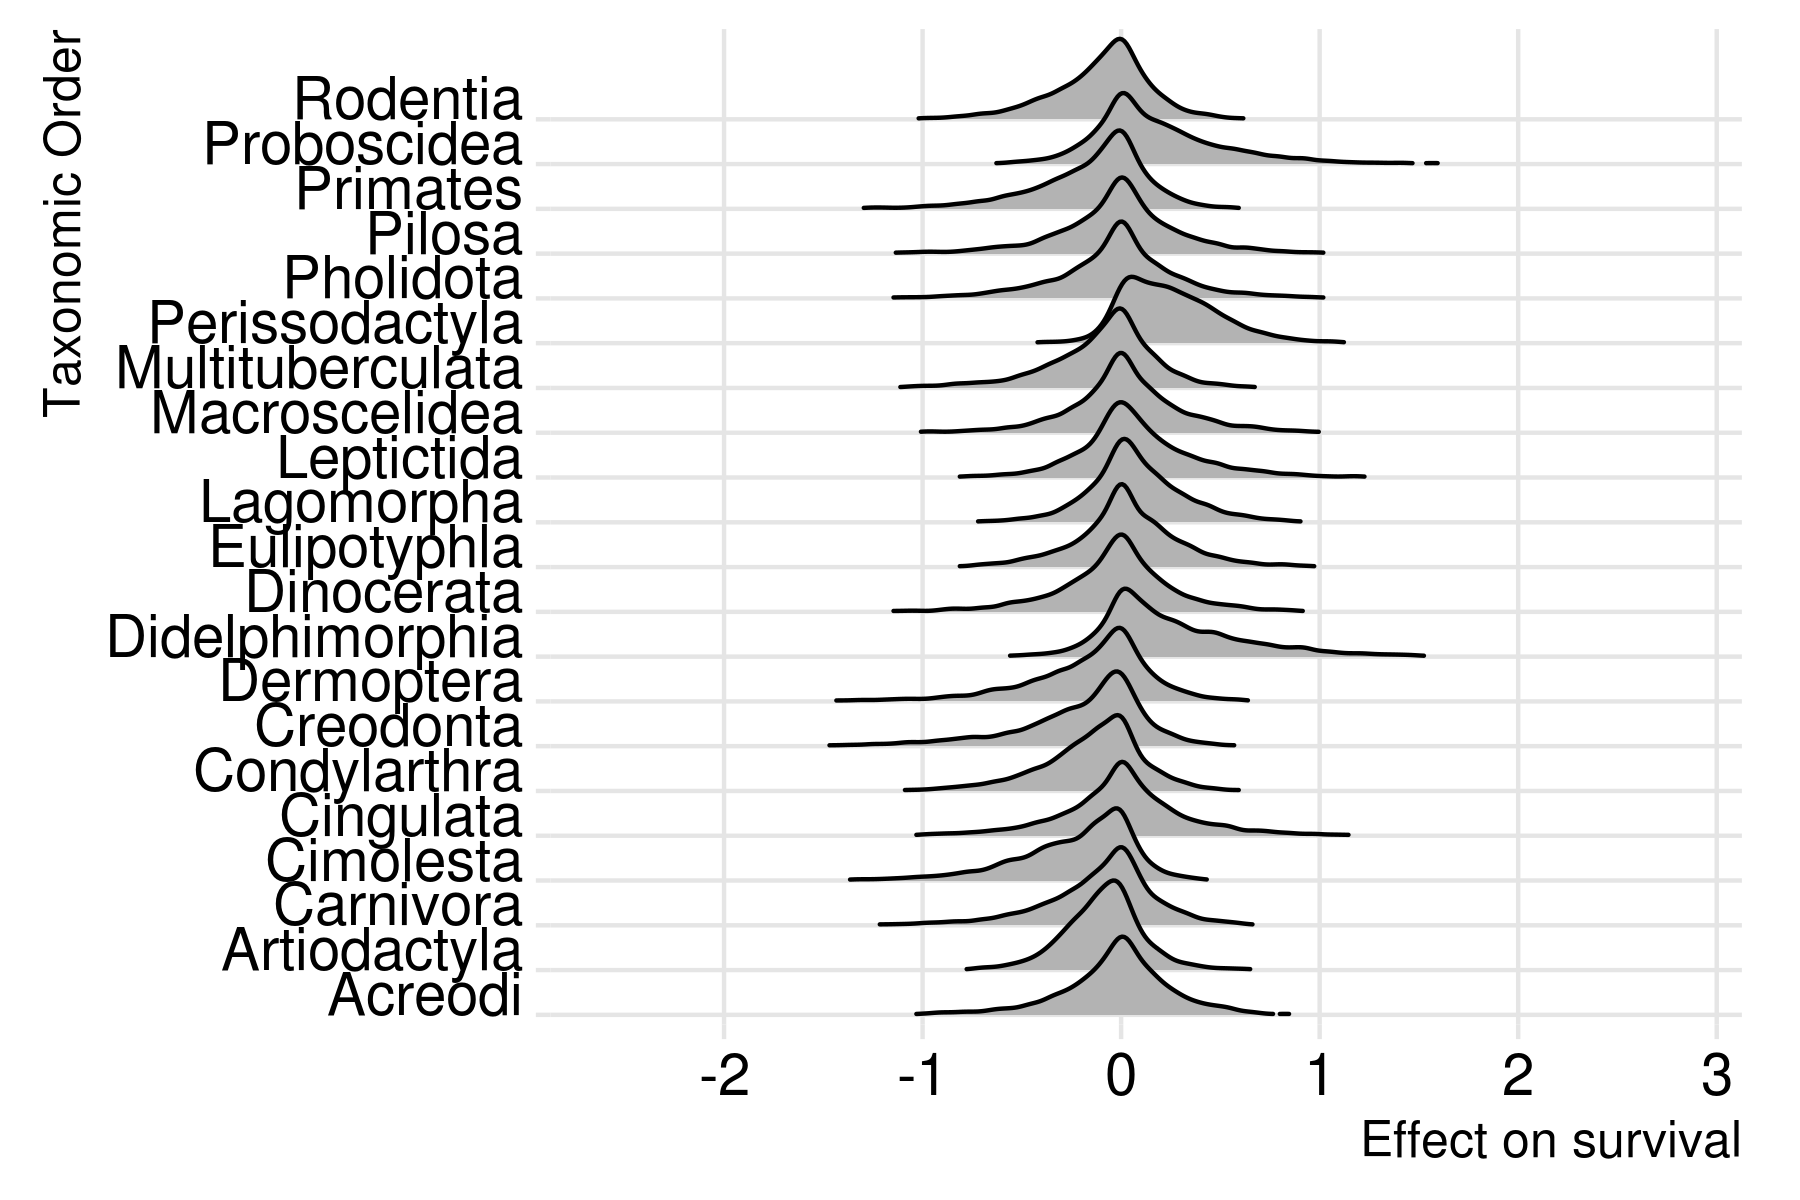
\includegraphics[width=\textwidth,height=0.4\textheight,keepaspectratio=true]{figure/order_survival_bd}
  \caption{Differences in log-odds of survival based on mammal orders. Positive values correspond to greater log-odds of survival than average, while negative values correspond to lower log-odds of survival than average.}
  \label{fig:order_surv}
\end{figure}

%     mass effect
Species mass is estimated to have no relationship or at best a weakly positive relationship with survival probability (Fig. \ref{fig:mass_survival}). This result means that differences in mass do not lead to differences in species survival. This result is consistent with previous studies of North American species and genus survival dynamics CITATION SMITS TOMIYA, and implies that other ecological factors have greater importance on survival than mass alone. \uppercase{get probability estimate}
\begin{figure}[ht]
  \centering
  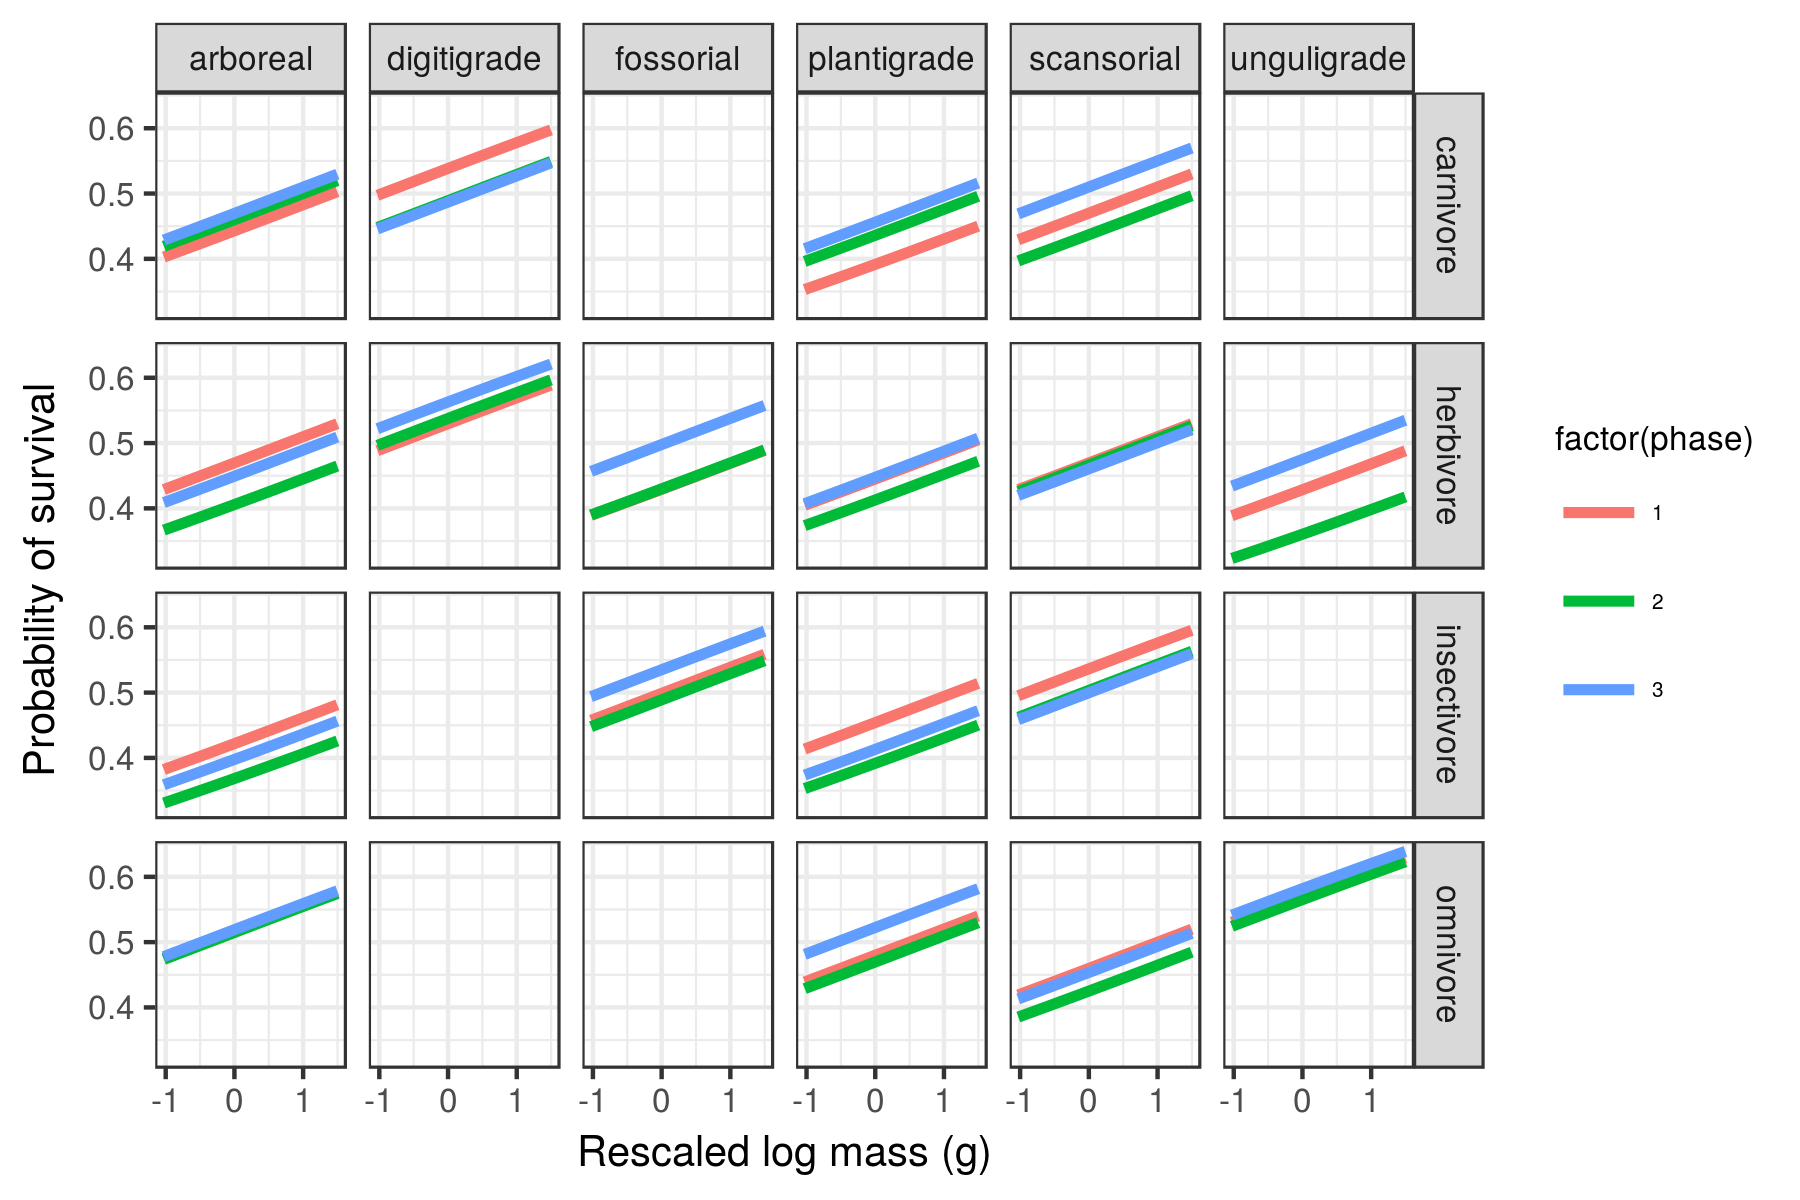
\includegraphics[width=\textwidth,height=0.4\textheight,keepaspectratio=true]{figure/mass_on_surv_bd}
  \caption[Effect of mass on probability of species survival as estimated from the birth-death model]{Mean estimate of the effect of species mass on the probability of a species survival for each of the three plant phases. The effect of mass is considered constant over time and that the only aspect of the model that changes with plant phase is the intercept of the relationship between mass and survival. The three plant phases are indicated by the color of the line. Mass has been log-transformed, centered, and rescaled; this means that a mass of 0 corresponds to the mean of log-mass of all observed species and that mass is in standard deviation units. For clarity, only the mean estimates of the effects of mass and plant plant are plotted.}
  \label{fig:mass_survival}
\end{figure}

%   group-level
%     temperature and plant phase
\begin{figure}[ht]
  \centering
  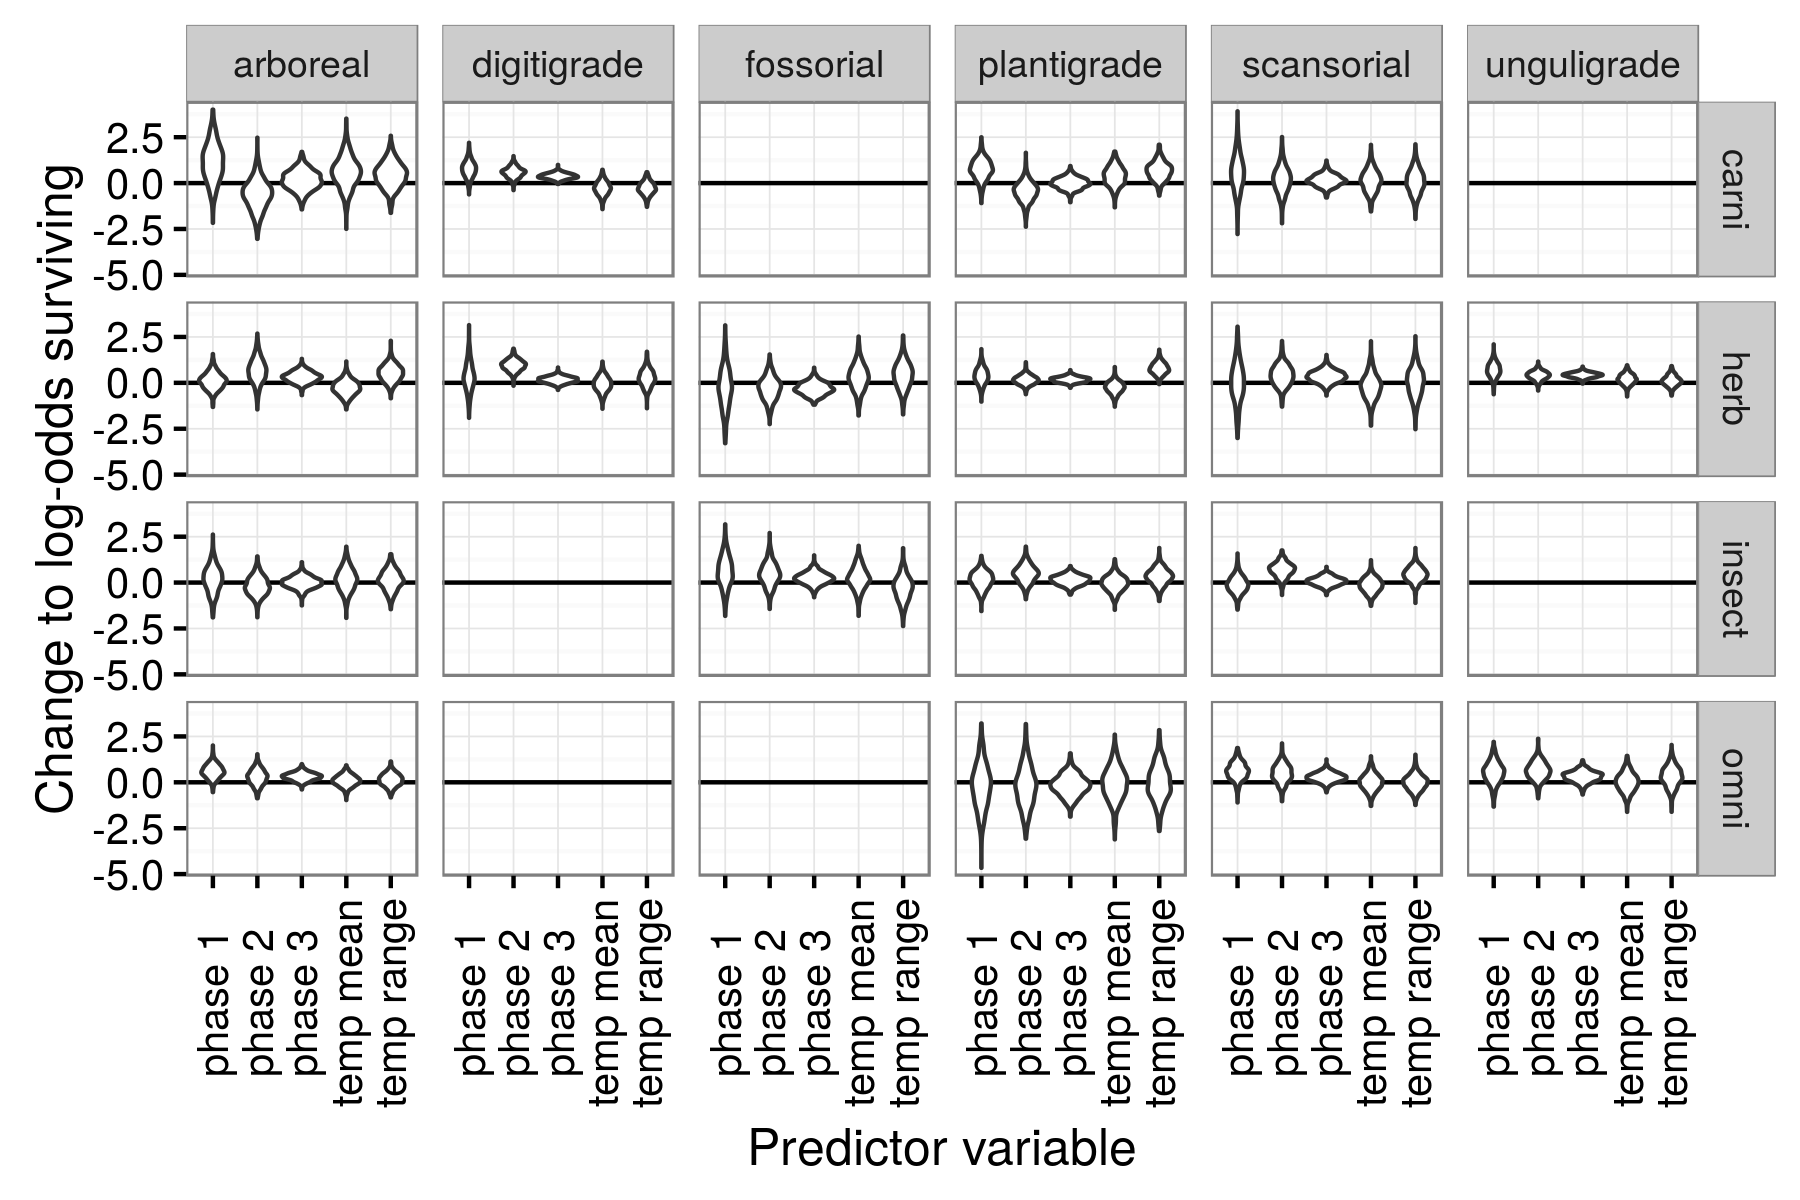
\includegraphics[width=\textwidth,height=0.4\textheight,keepaspectratio=true]{figure/group_on_survival_bd}
  \caption[Effects of group-level covariates on log-odds of ecotype survival as estimated from the birth-death model]{Estimated effects of the group-level covariates describing environmental context on log-odds of species survival. These estimates are from the birth-death model. What is plotted is a violin of the distribution of 1000 samples from the approximate posterior. The effect of plant phase graphed here is calculated as Phase 1\( = \gamma_{phase\ 1}\), Phase 2\( = \gamma_{phase\ 1} + \gamma_{phase\ 2}\), and so on.} 
  \label{fig:group_surv_bd}
\end{figure}


Functional group survival probability is rarely associated with differences between the three plant phases (Table \ref{tab:surv_plant}) with only five pair-wise comparisons having greater than 89\% probability of differences in survival between phases. Unuligrade herbivores have an approximately 89\% probability of having lower survival probability during the Paleocene-Eocene than the Miocene-Pleistocene. For digitgrade herbivores, and unguligrade ominvores, the Eocene-Miocene phase have an approximately 90\% probability of having greater survival probability than during the Micocene-Pleistocene phase. In contrast, unguligrade herbivores are estimated to have lower survival probability in the Eocene-Miocene phase than the Miocene-Pleistocene phase. Finally, unguligrade herbivores have an approximately 99\% probability of having a lower survival probability during the Paleocene-Eocene than the Eocene-Miocene.
\begin{table}[ht]
  \centering
  \caption[Posterior probablity estimates of differences in survival by plant phase]{Posterior probability of the differences in the log-odds of an ecotype surviving based on plant phase.} 
  \label{tab:surv_plant}
  \begin{tabular}{ l r r r }
    \hline
    & P(Eo.Mi $>$ 0) & P(Pa.Eo $>$ 0) & P(Eo.Mi $>$ Pa.Eo) \\ 
    \hline
    arboreal carnivore & 0.297 & 0.560 & 0.328 \\ 
    digitigrade carnivore & 0.786 & 0.367 & 0.743 \\ 
    plantigrade carnivore & 0.411 & 0.744 & 0.273 \\ 
    scansorial carnivore & 0.428 & 0.445 & 0.486 \\ 
    arboreal herbivore & 0.256 & 0.768 & 0.174 \\ 
    digitigrade herbivore & 1.000 & 0.400 & 0.942 \\ 
    fossorial herbivore & 0.696 & 0.563 & 0.565 \\ 
    plantigrade herbivore & 0.659 & 0.508 & 0.596 \\ 
    scansorial herbivore & 0.616 & 0.539 & 0.531 \\ 
    unguligrade herbivore & 0.000 & 0.102 & 0.012 \\ 
    arboreal insectivore & 0.289 & 0.483 & 0.368 \\ 
    fossorial insectivore & 0.532 & 0.420 & 0.592 \\ 
    plantigrade insectivore & 0.499 & 0.361 & 0.605 \\ 
    scansorial insectivore & 0.443 & 0.252 & 0.634 \\ 
    arboreal omnivore & 0.651 & 0.597 & 0.591 \\ 
    plantigrade omnivore & 0.417 & 0.549 & 0.393 \\ 
    scansorial omnivore & 0.486 & 0.525 & 0.487 \\ 
    unguligrade omnivore & 0.929 & 0.521 & 0.844 \\ 
    \hline
  \end{tabular}
\end{table}

Temperature is estimated to have no effect on functional group survival probability (Table \ref{tab:surv_temp}). 
\begin{table}[ht]
  \centering
  \caption[Posterior probablity of effects of temperature on survival]{Posterior probability that the effects of the two temperature covariates on the log-odds of an ecotype survival are greater than 0. What is estimated is the probability that these estimates are greater than 0; high or low probabilities indicate the ``strength'' of the covariate in that direction (positive and negative, respectively). These estimates are from the birth-death model.}
  \label{tab:surv_temp}
  \begin{tabular}{ l r r }
    \hline
    & \(P(\gamma_{temp\ mean} > 0)\) \\
    \hline
    arboreal carnivore & 0.665 \\ 
    digitigrade carnivore & 0.453 \\ 
    plantigrade carnivore & 0.618 \\ 
    scansorial carnivore & 0.380 \\ 
    arboreal herbivore & 0.761 \\ 
    digitigrade herbivore & 0.395 \\ 
    fossorial herbivore & 0.429 \\ 
    plantigrade herbivore & 0.279 \\ 
    scansorial herbivore & 0.345 \\ 
    unguligrade herbivore & 0.818 \\ 
    arboreal insectivore & 0.489 \\ 
    fossorial insectivore & 0.452 \\ 
    plantigrade insectivore & 0.435 \\ 
    scansorial insectivore & 0.384 \\ 
    arboreal omnivore & 0.600 \\ 
    plantigrade omnivore & 0.639 \\ 
    scansorial omnivore & 0.512 \\ 
    unguligrade omnivore & 0.396 \\ 
    \hline
  \end{tabular}
\end{table}

%     correlation
\begin{figure}[ht]
  \centering
  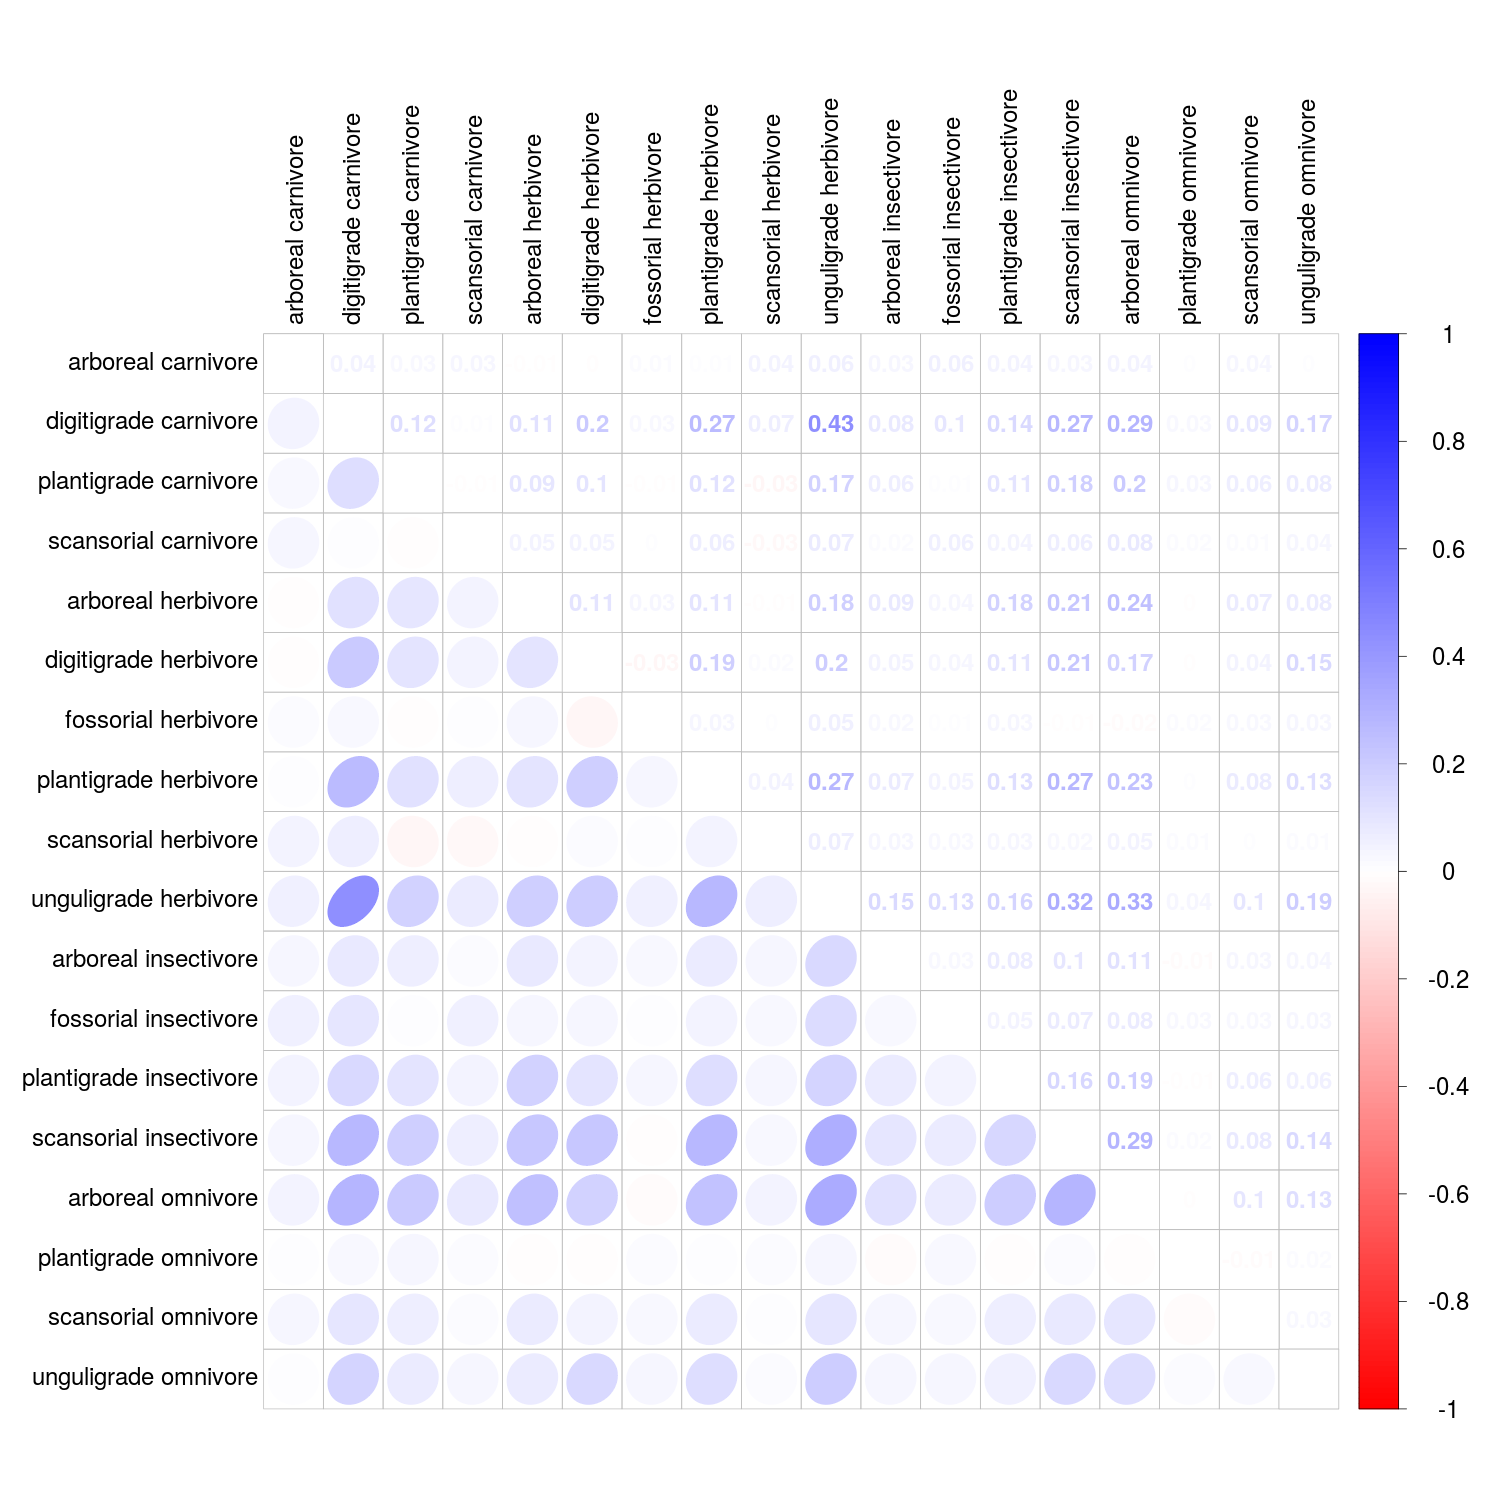
\includegraphics[width=\textwidth,height=\textheight,keepaspectratio=true]{figure/survival_correlation}
  \caption[Estimated correlations in survival probability between ecotypes]{Posterior mean estimates of the correlations in survival probability between the mammal ecotypes. The lower triangle of the matrix is populated with ellipses corresponding to the level of correlation between the two ecotypes, while the upper triangle of the matrix corresponds to the mean estimated correlation between ecotypes. Darker values correspond to a greater magnitude of correlation with blue values corresponding to a positive correlation and red values a negative correlation.}
  \label{fig:survival_corr}
\end{figure}







\subsection*{Analysis of diversity}

All of the analyses of diversification and macroevolutionary rates has been done using only the birth-death model because of the model's better posterior predictive check performance (Fig. \ref{fig:ppc}).


The general pattern of the estimated North American total mammal diversity for the Cenozoic is ``stable'' in that diversity fluctuates around a constant mean standing diverisity, does not fluctuate wildly and rapidly over the Cenozoic, and demonstrates no sustained directional trends (Fig. \ref{fig:diversity_est}). In broad strokes, the first 15 or so million years of the Cenozoic are characterized by first an increase and then a decline in standing diversity at approximately 45-50 Mya (early-middle Eocene). Following this decline, standing diversity is broadly constant from 45 to 18 Mya (early Miocene). After this, there is a rapid spike in diversity followed by a slight decline in diversity up to the Recent. 

The pattern exhibited by the diversity history estimated in this study (Fig. \ref{fig:diversity_est}) has some major similarities with previous mammal diversity curves \citep{Alroy2009}: both curves begin with an increase in diversity most of the major increases in diversity are retained including the large diversity spike during the Miocene. Unlike subsampling based approaches to estimating diversity \citep{Alroy2010c}, I'm able to interpolate over unsampled/poorly sampled time periods because of how the hierarchical model can share information across the different units \cite{Gelman2013d}; for cases like unsampled temporal bins, this may lead to estimates with high uncertainty, but that is preferable to no estimate at all. Finally, the Bayesian framework here gives a distribution of possible estimates of diversity allowing for direct inspection of the uncertainty of our inferences, something that is preferable to both traditional and resampling based confidence interval estimates \citep{Gelman2013d}. Note that my time series of estimated diversity begins at a slightly different point than that of \citet{Alroy2009} and that the time intervals used by \citet{Alroy2009} are slightly shorter than those used here, so this may cause some of the minor differences between the curves. Also, please note that the diversity values are plotted at the ``ceiling'' of each temporal interval and not at the midpoint (Fig. \ref{fig:diversity_est}).

When viewed through the lens of diversification rate, some of the structure behind the estimated diversity history begins to take shape (Fig. \ref{fig:diversity_rate}). For most of the Cenozoic, the diversification rate hovers around zero, punctuated by both positive and negative spikes. The largest spike in diversification rate is at 16 Mya, which is early Oligocene (Fig. \ref{fig:diversity_rate}). Other notable increases in diversification rate occur 56, 46, 22, 18, and 6 Mya (Table \ref{tab:div_peak}), though the last of these may be due to edge effects surrounding the partial-identifiability of \(p_{t = T}\). Notable decreases in diversification rate occur at 54, 50, 48, 44, 40, 34, 30, 24, 20, 16, 12, and 8 Mya (Table \ref{tab:div_peak}), meaning that diversification rate has more major decreases than increases. While diversification rates significantly lower than average are more common than diversification rates greater than average, when diversification rate does increases it is with a greater magnitude than most decreases (Fig. \ref{fig:diversity_rate}). Given that diversification rate more closely resembles origination rate than extinction rate (Fig. \ref{fig:diversity_rate}, \ref{fig:origin_rate}, \ref{fig:extinct_rate}), these decreases in diversification rate may be indicative of ``depletions'' (failure to replace extinct taxa) rather than pulses of extinction. 

The estimates from this study of per capita origination and extinction rates for the entire species pool (Fig. \ref{fig:origin_rate}, \ref{fig:extinct_rate}) are very different from the origination and extinction rates estimated by \citet{Alroy2009}. The two most striking difference are the very different estimates of extinction rate between the two studies and the very different scales of the origination rate estimates. This may be due to the fundamentally different way these rates are calculated, and how the diversification process was modeled. The per capita rates estimated in this study follow straight from the definition of a per capita rate (e.g. number of originations between time \(t\) and \(t + 1\) divided by the diversity at time \(t\)) while the rates calculated in \citet{Alroy2009} are based on log ratios of standing diversity.

The comparison between per capita origination and extinction rate estimates reveals how diversification rate is formed (Fig. \ref{fig:origin_rate}, \ref{fig:extinct_rate}). As expected given previous inspection of the ecotype specific estimates of origination and survival probabilities from the birth-death model, diversification rate seems most driven by changes in origination rate as opposed to extinction rate. Extinction rate, on the other hand, demonstrates an almost saw-toothed pattern around a constant mean (Fig. \ref{fig:extinct_rate}). These results are broadly consistent with those from previous analyses of North American mammals diversity and diversification \citep{Alroy1996a,Alroy2000g,Alroy2009}.


\begin{figure}[ht]
  \begin{subfigure}[b]{0.45\textwidth}
    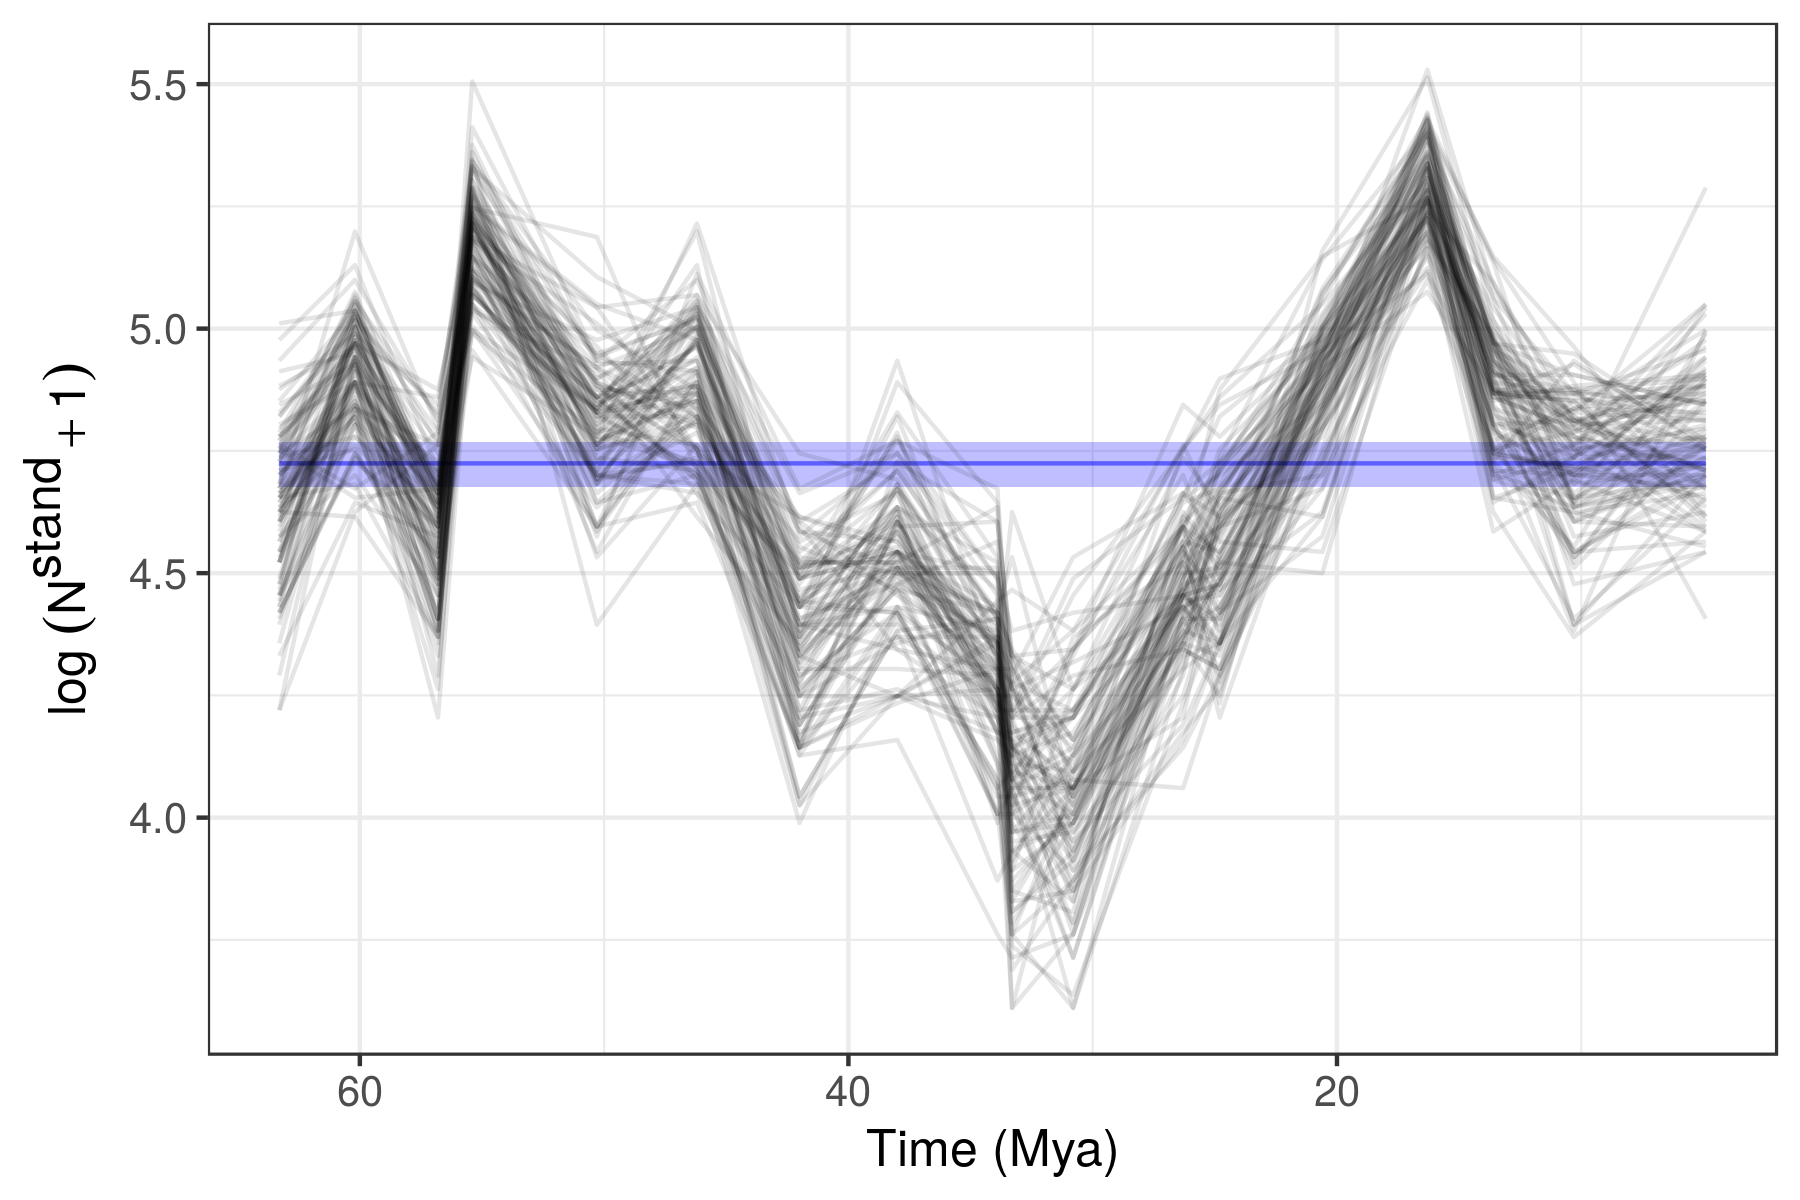
\includegraphics[width=\textwidth,height=0.5\textheight,keepaspectratio=true]{figure/log_diversity}
    \caption{Log diversity}
    \label{fig:diversity_est}
  \end{subfigure}
  \begin{subfigure}[b]{0.45\textwidth}
    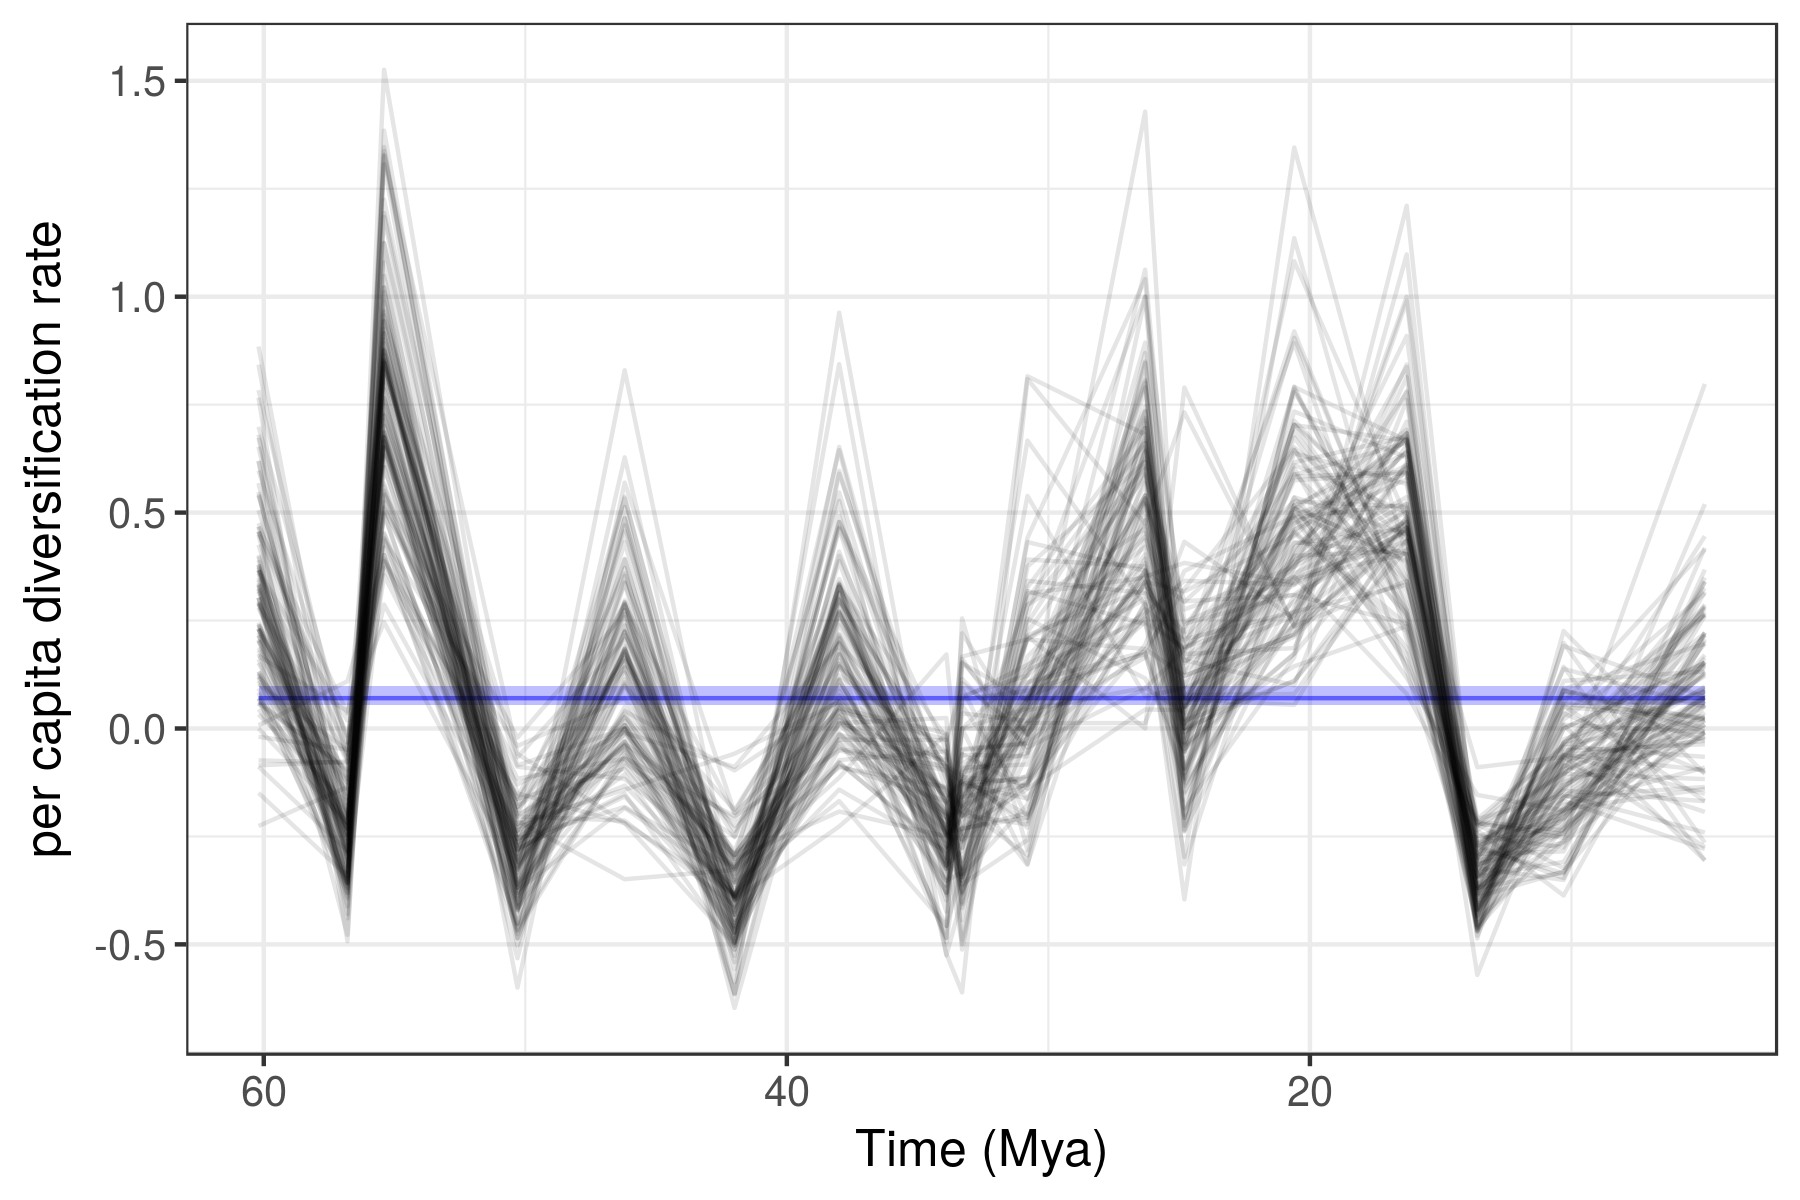
\includegraphics[width=\textwidth,height=0.5\textheight,keepaspectratio=true]{figure/div_rate}
    \caption{Diversification rate}
    \label{fig:diversity_rate}
  \end{subfigure}
  \caption[Estimated mammal log-diversity and macroevolutionary rates for the Cenozoic]{Posterior estimates of the time series of Cenozoic North American mammal diversity and it's characteristic macroevolutionary rates; all estimates are from the birth-death model and 100 posterior draws are plotted to indicate the uncertainty in these estimates. The blue horizontal strip corresponds to the 80\% credible interval of estimated mean standing diversity, diversification rate, origination rate, and extinction rate respectively; the median estimate is also indicated. What is also plotted is the  The dramatic differences between diversity estimates at the first and second time points and the penultimate and last time points in this series are caused by well known edge effects in discrete-time birth-death models caused by \(p_{\_, t = 1}\) and \(p_{\_, t = T}\) being partially unidentifiable \citep{Royle2008}; the hierarchical modeling strategy used here helps mitigate these effects but they are still present \citep{Gelman2013d,Royle2008}. Diversification rate is in units of species gained per species present per time unit (2 My), origination rate is in units of species originating per species present per time unit, and extinction rate is in units of species becoming extinct per species present per time unit.}
  \label{fig:macro_values}
\end{figure}

\begin{table}[ht]
  \centering
  \caption[Posterior probability estimates of a peak in diversity, diversification]{Posterior probabilities of diversity \(N^{stand}_{t}\) or diversification rate \(D^{rate}_{t}\) being greater than average standing diversity \(\overline{N^{stand}}\) or average diversification rate \(\overline{D^{rate}}\) for the whole Cenozoic. The ``Time'' column corresponds to the top of each of the temporal bins. Diversification rate can not be estimated for the last time point because it is unknown how many more species originated or went extinct following this temporal bin. The estimates are from the birth-death model.}
  \label{tab:div_peak}
  \begin{tabular}{ r r r }
    \hline
    NALMA & \(P(N^{stand}_{t} > \overline{N^{stand}})\) & \(P(D^{rate}_{t} > \overline{D^{rate}})\) \\ 
    \hline
    Torrejonian & 0.79 & \\ 
    Tiffanian & 0.95 & 0.67 \\ 
    Clarkforkian & 0.50 & 0.03 \\ 
    Wasatchian & 1.00 & 0.99 \\ 
    Bridgerian & 0.69 & 0.00 \\ 
    Uintan & 0.75 & 0.45 \\ 
    Duchesnean & 0.00 & 0.00 \\ 
    Chadronian & 0.01 & 0.70 \\ 
    Orellan & 0.00 & 0.01 \\ 
    Whitneyan & 0.00 & 0.09 \\ 
    Geringian & 0.00 & 0.57 \\ 
    Monroecreekian & 0.01 & 1.00 \\ 
    Harrisonian & 0.11 & 0.67 \\ 
    Hemingfordian & 0.96 & 0.99 \\ 
    Barstovian & 1.00 & 1.00 \\ 
    Clarendonian & 0.93 & 0.00 \\ 
    Hemphillian & 0.63 & 0.10 \\ 
    Blancan & 0.73 & 0.43 \\ 
    \hline
  \end{tabular}
\end{table}


Diversity partitioned by ecotype reveals a lot of the complexity behind the pattern of mammal diversity for the Cenozoic (Fig. \ref{fig:ecotype_diversity}). 

\begin{figure}[ht]
  \centering
  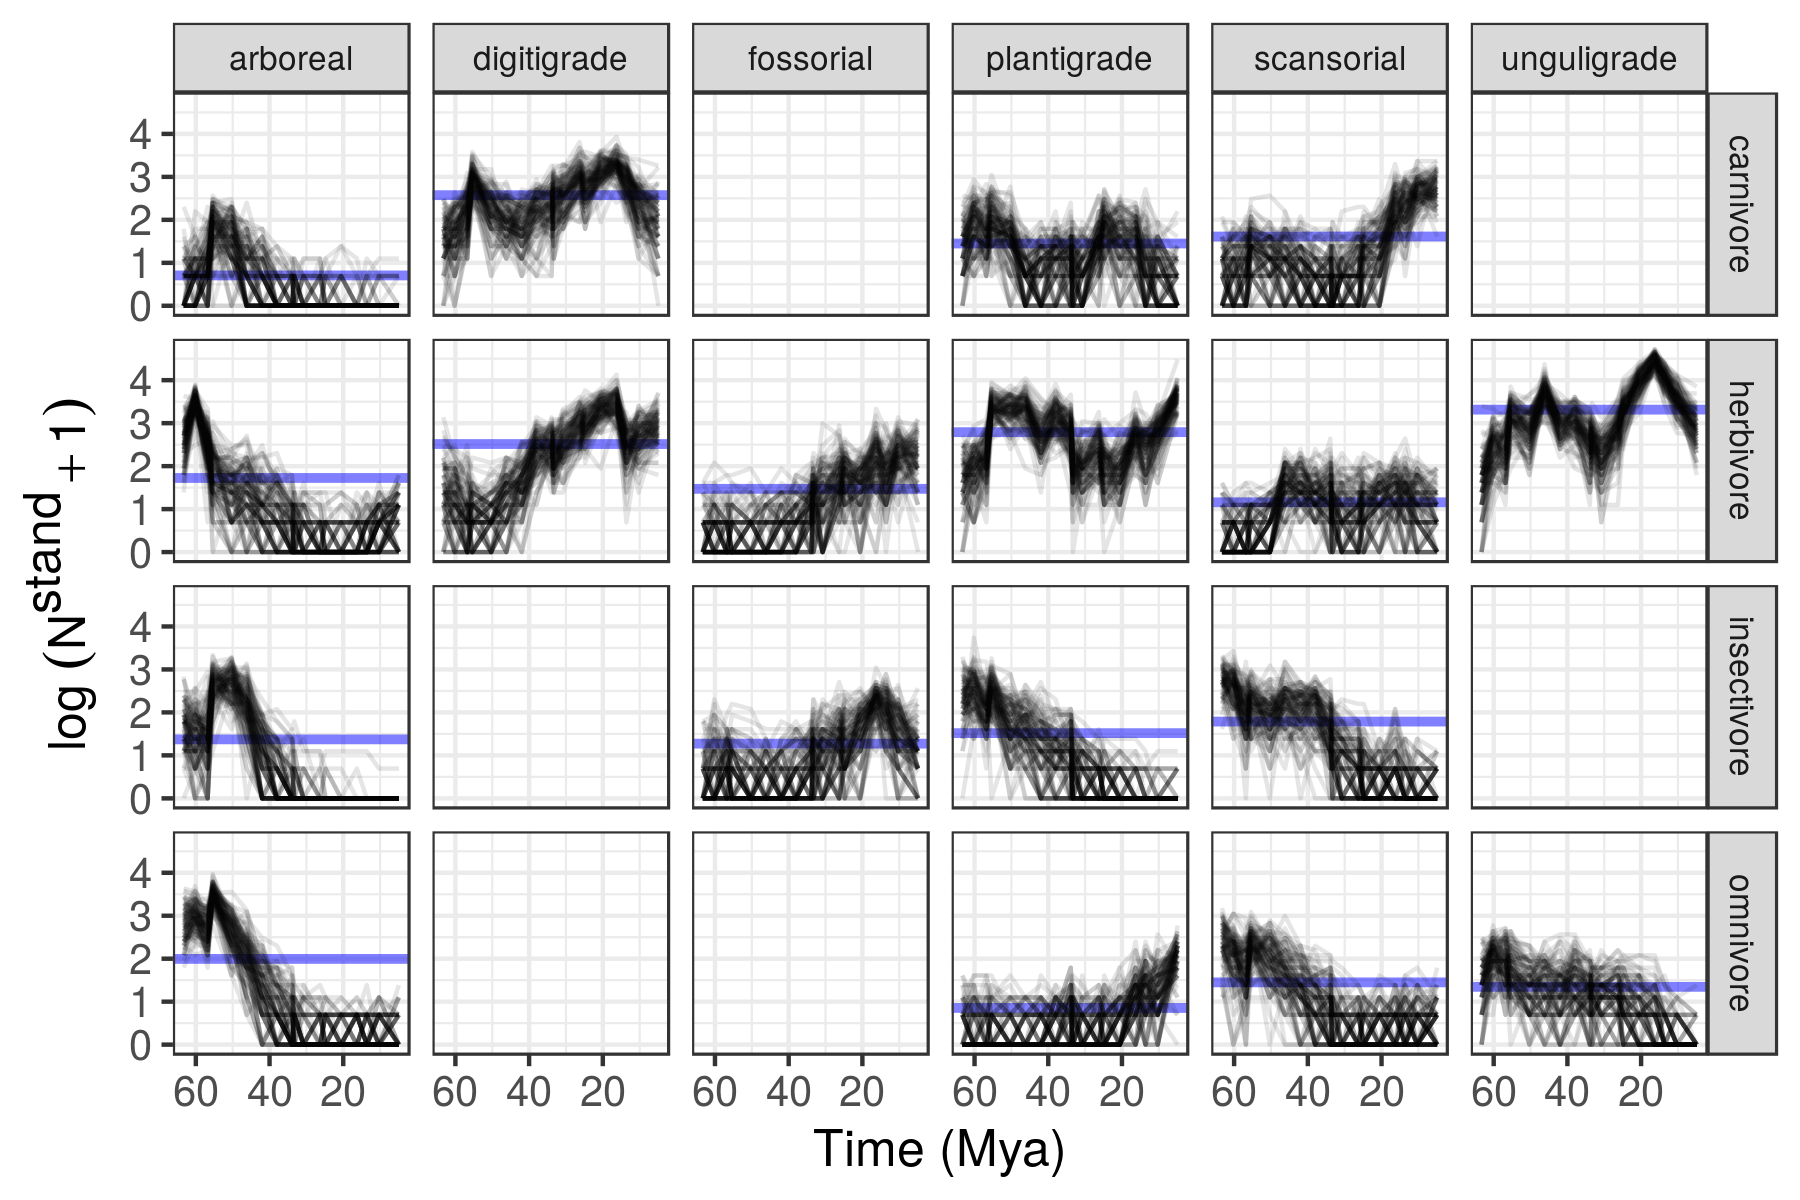
\includegraphics[width=\textwidth,height=0.5\textheight,keepaspectratio=true]{figure/ecotype_diversity}
  \caption[Estimated mammal ecotype log-diversity for the Cenozoic]{Posterior of standing log-diversity of North American mammals by ecotype for the Cenozoic as estimated from the birth-death model; 100 posterior draws are plotted to indicate the uncertainty in these estimates and what is technically plotted is log of diversity plus 1.}
  \label{fig:ecotype_diversity}
\end{figure}

Arboreal ecotypes obtain peak diversity early in the Cenozoic and then decline for the rest of the time series, becoming increasingly rare or absent as diversity approaches the Recent (Fig. \ref{fig:ecotype_diversity}). Arboreal herbivores and omnivores obtain peak diversity at the beginning of the Cenozoic then go into decline while remaining a small part of the species pool, while arboreal carnivores and insectivores obtain peak diversity 52-50 Mya and then quickly decline and become extremely rare or entirely absent from the species pool. This is consistent with increasing extinction risk in the Neogene compared to the Paleogene as proposed by \citet{Smits2015b}.

The diversity of digitigrade and unguligrade herbivores increases over the Cenozoic (Fig. \ref{fig:ecotype_diversity}). In contrast, plantigrade herbivore diversity does not have a single, broad-strokes pattern; instead, diversity increases, decreases, and may have then increased till the Recent. In contrast, fossorial and scansorial herbivores demonstrate a much flatter history of diversity, with a slight increase in diversity that over time is more pronounced among fossorial taxa than scansorial taxa. The expansion of digitigrade and unguligrade herbivores over the Cenozoic is consistent with the gradual expansion of grasslands which these ecotypes are better adapted to than closed environments \citep{Blois2009,Stromberg2005}.

Digitigrade carnivores have a multi-modal diversity history, with peaks at 54-52 and 12-10 Mya (Fig.\ref{fig:ecotype_diversity}). Between these two peaks digitigrade carnivore diversity dips below average diversity following the first peak and then grows slowly until the second peak. Plantigrade carnivores obtain peak diversity in the early Cenozoic and then maintain a relatively stable diversity until another peak at the end of the Cenozoic. The generally flat diversity history digitigrade carnivores lacks any sustained temporal trends and seems to reflect previous findings of limited diversity in spite of constant turnover and morphological evolution \citep{Valkenburgh1999,Silvestro2015b,Slater2015c}

There are some broad similarities in diversity histories of insectivorous and omnivorous taxa. The diversity histories of arboreal, plantigrade, and scansorial insectivorous taxa all demonstrate a decreasing pattern with time, while fossorial insectivores have a flat diversity history with a peak approximately 10 Mya (Fig. \ref{fig:ecotype_diversity}). Arboreal and scansorial omnivores decrease in diversity from their initial peaks early in the Cenozoic, and plantigrade omnivores have a generally flat diversity history with a sudden peak in diversity late in the Cenozoic (Fig. \ref{fig:ecotype_diversity}). Unguligrade omnivores also demonstrate a possible decrease in diversity over the Cenozoic, but not as clearly as arboreal and scansorial omnivores.


The waxing and waning of the mammal ecotypes is obvious when comparing changes to estimated relative log-mean of diversity (Fig. \ref{fig:ecotype_relative}). While ecotype diveristy does appear to change gradually, there are definite changes to the relative contributions of the ecotypes to the regional species pool. All arboreal ecotypes clearly decrease in relative diversity over the Cenozoic. In contrast the the digitigrade herbivore, fossorial herbivore, scansorial herbivore, and unguligrade herbivore ecotypes which increase in relative diversity over the Cenozoic. The digitigrade carnivore ecotype increases in relative diveristy until approximately the start of the Neogene, after which it maintains a generally constant relative diveristy; this is consistent with previous observations of constant or density-dependent diversity of the canid guild for the Neogene \citep{Valkenburgh1999,Silvestro2015b,Slater2015c}, a guild that overlaps with the digitigrade carnivore ecotype. Plantigrade herbivores remain a constant relative contribution to ecotypic diveristy. These results support the hypothesis of a gradual transition from the early Paleogene with a region with more avaliable habitat for aboreal taxa and less avaliable habitat for many digitigrade and unguligrade taxa, to an environment where arboreal taxa are absent from the species pool and digitigrade and unguligrade taxa are much more dominant (Fig. \ref{fig:ecotype_relative}). It is the relative contributions of digitgrade carnivores, digitigrade herbivores, and unguligrade herbivores which really shape the regional species pool of the Neogene. 


\begin{figure}[ht]
  \centering
  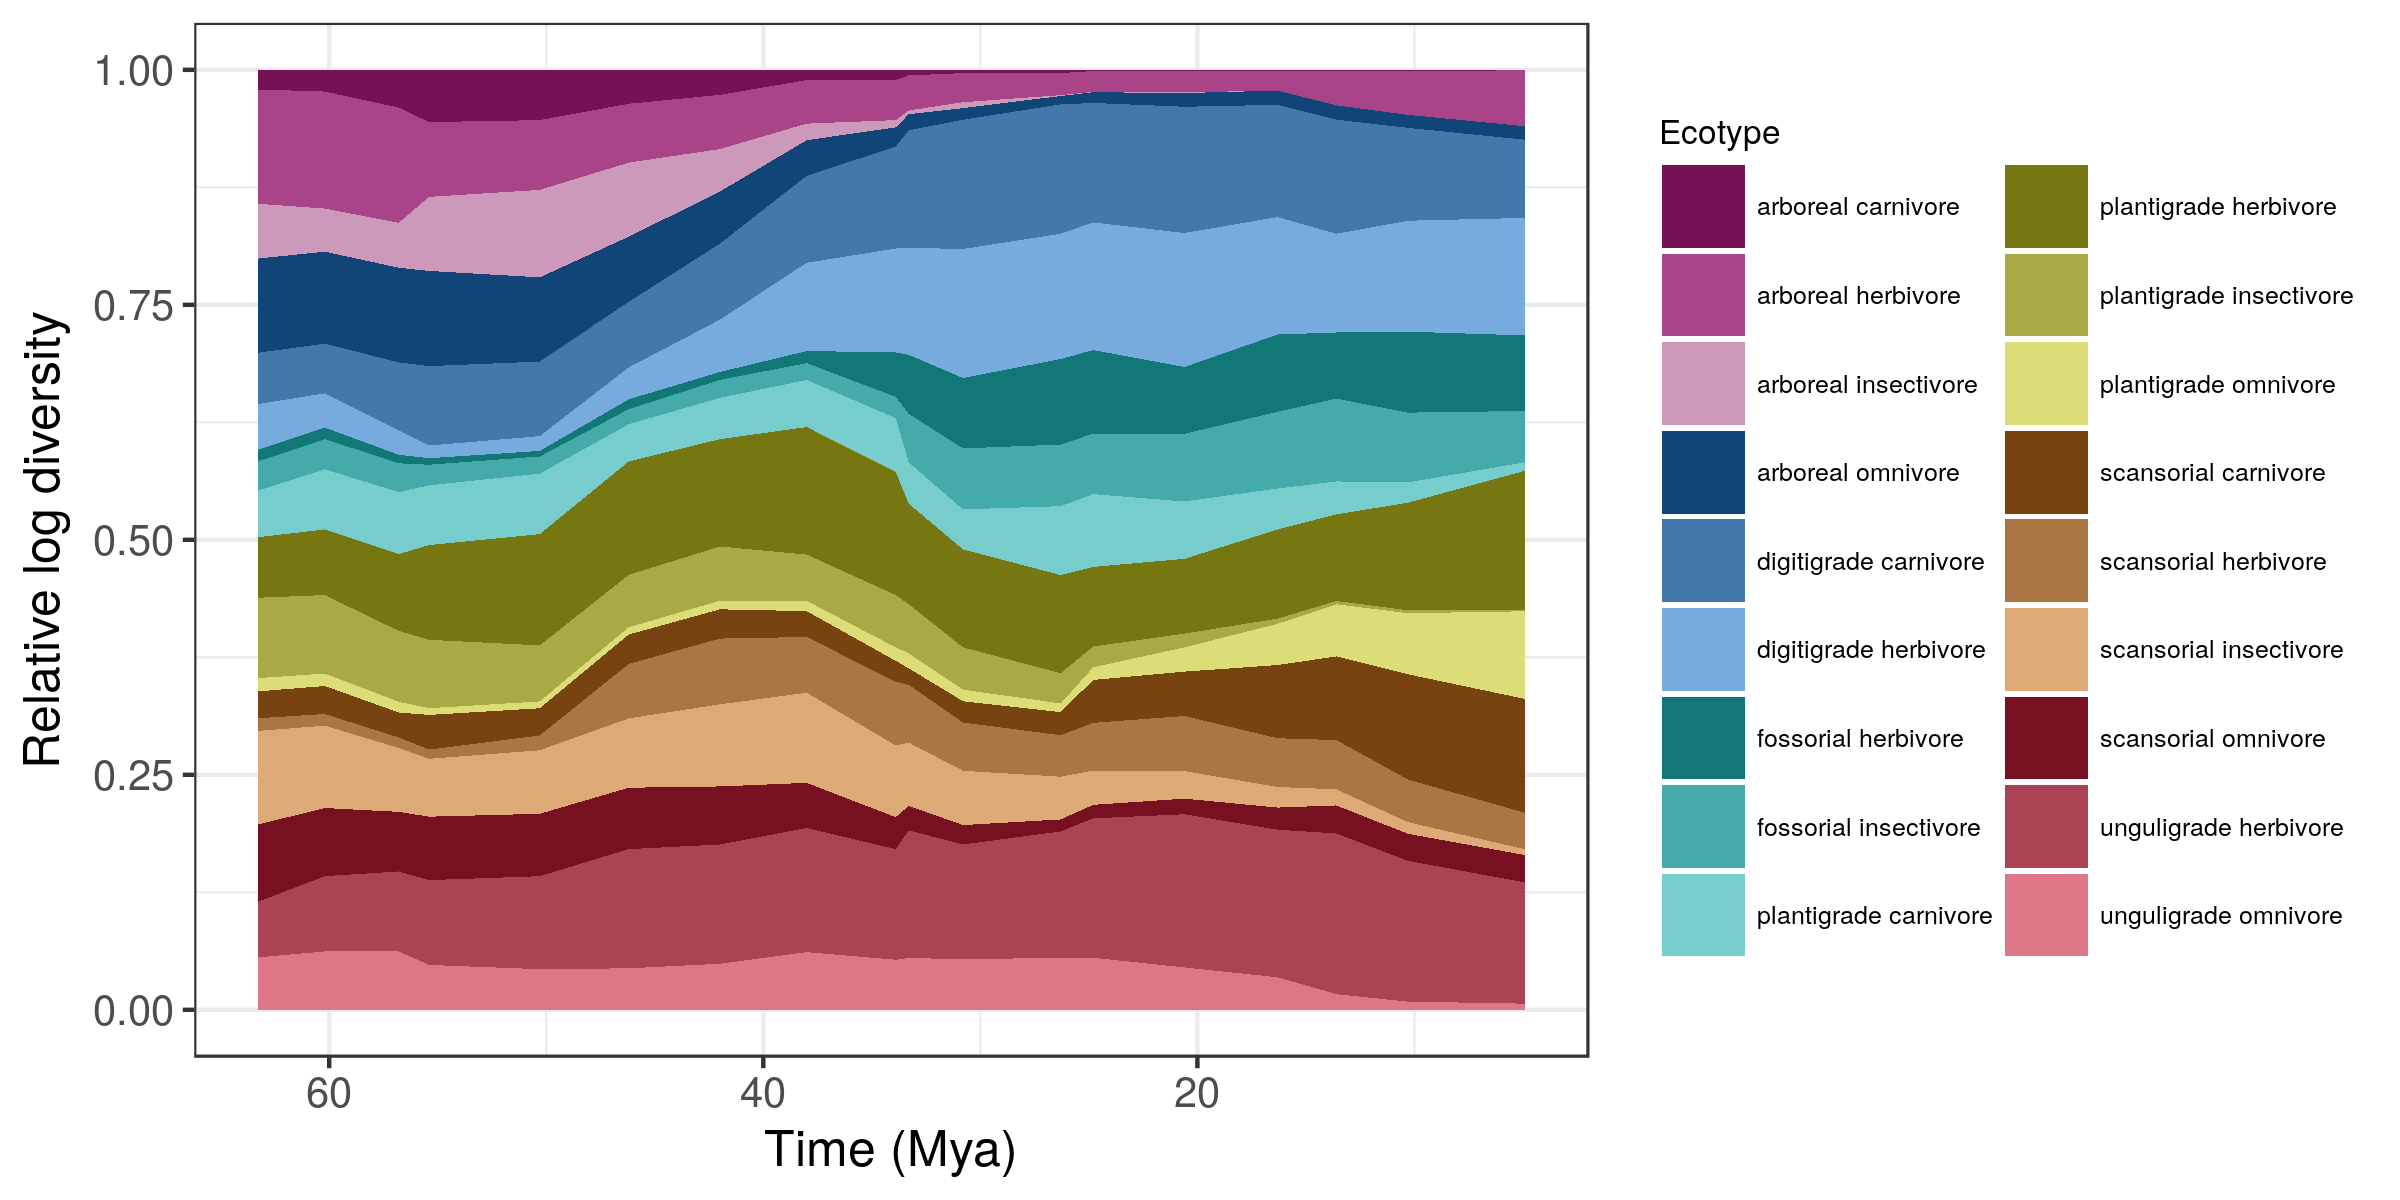
\includegraphics[width=\textwidth,height=0.5\textheight,keepaspectratio=true]{figure/relative_diversity}
  \caption[Relative mammal ecotype log-diversity for the Cenozoic]{Mean posterior estimate of relative log standing diveristy of 18 North American mammal ecotypes for the Cenozoic. These estimates are calculated from 100 posterior estimates of the true occurrence matrix \(z\) as estimated from the birth-death model.}
  \label{fig:ecotype_relative}
\end{figure}


Many of the estimated ecotype-specific diversity histories share a similar increase in diversity in the late Cenozoic, 16-14 Mya (Fig. \ref{fig:ecotype_diversity}). These increases are either sustained or temporary and are seen in digitigrade carnivores, plantigrade carnivores, scansorial carnivores, unguligrade herbivores, fossorial insectivores, and plantigrade omnivores.



\end{document}

